% Options for packages loaded elsewhere
\PassOptionsToPackage{unicode}{hyperref}
\PassOptionsToPackage{hyphens}{url}
%
\documentclass[
]{article}
\usepackage{amsmath,amssymb}
\usepackage{lmodern}
\usepackage{iftex}
\ifPDFTeX
  \usepackage[T1]{fontenc}
  \usepackage[utf8]{inputenc}
  \usepackage{textcomp} % provide euro and other symbols
\else % if luatex or xetex
  \usepackage{unicode-math}
  \defaultfontfeatures{Scale=MatchLowercase}
  \defaultfontfeatures[\rmfamily]{Ligatures=TeX,Scale=1}
\fi
% Use upquote if available, for straight quotes in verbatim environments
\IfFileExists{upquote.sty}{\usepackage{upquote}}{}
\IfFileExists{microtype.sty}{% use microtype if available
  \usepackage[]{microtype}
  \UseMicrotypeSet[protrusion]{basicmath} % disable protrusion for tt fonts
}{}
\makeatletter
\@ifundefined{KOMAClassName}{% if non-KOMA class
  \IfFileExists{parskip.sty}{%
    \usepackage{parskip}
  }{% else
    \setlength{\parindent}{0pt}
    \setlength{\parskip}{6pt plus 2pt minus 1pt}}
}{% if KOMA class
  \KOMAoptions{parskip=half}}
\makeatother
\usepackage{xcolor}
\usepackage[margin=1in]{geometry}
\usepackage{graphicx}
\makeatletter
\def\maxwidth{\ifdim\Gin@nat@width>\linewidth\linewidth\else\Gin@nat@width\fi}
\def\maxheight{\ifdim\Gin@nat@height>\textheight\textheight\else\Gin@nat@height\fi}
\makeatother
% Scale images if necessary, so that they will not overflow the page
% margins by default, and it is still possible to overwrite the defaults
% using explicit options in \includegraphics[width, height, ...]{}
\setkeys{Gin}{width=\maxwidth,height=\maxheight,keepaspectratio}
% Set default figure placement to htbp
\makeatletter
\def\fps@figure{htbp}
\makeatother
\setlength{\emergencystretch}{3em} % prevent overfull lines
\providecommand{\tightlist}{%
  \setlength{\itemsep}{0pt}\setlength{\parskip}{0pt}}
\setcounter{secnumdepth}{-\maxdimen} % remove section numbering
\newlength{\cslhangindent}
\setlength{\cslhangindent}{1.5em}
\newlength{\csllabelwidth}
\setlength{\csllabelwidth}{3em}
\newlength{\cslentryspacingunit} % times entry-spacing
\setlength{\cslentryspacingunit}{\parskip}
\newenvironment{CSLReferences}[2] % #1 hanging-ident, #2 entry spacing
 {% don't indent paragraphs
  \setlength{\parindent}{0pt}
  % turn on hanging indent if param 1 is 1
  \ifodd #1
  \let\oldpar\par
  \def\par{\hangindent=\cslhangindent\oldpar}
  \fi
  % set entry spacing
  \setlength{\parskip}{#2\cslentryspacingunit}
 }%
 {}
\usepackage{calc}
\newcommand{\CSLBlock}[1]{#1\hfill\break}
\newcommand{\CSLLeftMargin}[1]{\parbox[t]{\csllabelwidth}{#1}}
\newcommand{\CSLRightInline}[1]{\parbox[t]{\linewidth - \csllabelwidth}{#1}\break}
\newcommand{\CSLIndent}[1]{\hspace{\cslhangindent}#1}
\usepackage{caption} \captionsetup{font={footnotesize},width=6in} \renewcommand{\dblfloatpagefraction}{.9} \makeatletter \renewenvironment{figure} {\def\@captype{figure}} \makeatletter
\ifLuaTeX
  \usepackage{selnolig}  % disable illegal ligatures
\fi
\IfFileExists{bookmark.sty}{\usepackage{bookmark}}{\usepackage{hyperref}}
\IfFileExists{xurl.sty}{\usepackage{xurl}}{} % add URL line breaks if available
\urlstyle{same} % disable monospaced font for URLs
\hypersetup{
  hidelinks,
  pdfcreator={LaTeX via pandoc}}

\author{}
\date{\vspace{-2.5em}}

\begin{document}

\hypertarget{mcnebula-critical-chemical-classes-to-classify-and-boost-identification-by-visualization-for-untargeted-lc-msms-data-analysis}{%
\section{MCnebula: Critical chemical classes to classify and boost
identification by visualization for untargeted LC-MS/MS data
analysis}\label{mcnebula-critical-chemical-classes-to-classify-and-boost-identification-by-visualization-for-untargeted-lc-msms-data-analysis}}

\textbf{Lichuang Huang\textsuperscript{1,~2~\#}, Qiyuan
Shan\textsuperscript{1,~2~\#},} \textbf{Qiang Lyu\textsuperscript{1},
Shuosheng Zhang\textsuperscript{3}, Lu Wang\textsuperscript{1,~2*}, Gang
Cao\textsuperscript{1,~2*}}

\textsuperscript{1} School of Pharmacy, Zhejiang Chinese Medical
University, Hangzhou, China

\textsuperscript{2} Jinhua Institute, Zhejiang Chinese Medical
University, Hangzhou, China

\textsuperscript{3} College of Chinese Materia Medica and Food
Engineering, Shanxi University of Chinese Medicine, Jinzhong, China.

\textsuperscript{\#}These authors contributed equally to this work

*Address correspondence to:

\textbf{Lu Wang, Ph.D.}

School of Pharmacy, Zhejiang Chinese Medical University, No.~548 Binwen
Road, Hangzhou, Zhejiang 310053, China; E-mail:
\href{mailto:luwang0520@163.com}{\nolinkurl{luwang0520@163.com}}

\textbf{Professor Gang Cao, Ph.D.}

School of Pharmacy, Zhejiang Chinese Medical University, No.~548 Binwen
Road, Hangzhou, Zhejiang 310053, China; Tel/Fax: +86 571 87195895;
E-mail: \href{mailto:caogang33@163.com}{\nolinkurl{caogang33@163.com}}

\hypertarget{abstract}{%
\subsection{Abstract}\label{abstract}}

Untargeted mass spectrometry is a robust tool for biology, but it
usually requires much time on data analysis especially for system
biology. We established a framework called MCnebula (Multiple-Chemical
nebula) to facilitate mass spectrometry data analysis process by
focusing on critical chemical classes and visualization in multiple
dimensions. It consisted of three vital steps: (1) abundance-based
classes (ABC) selection algorithm, (2) critical chemical classes to
classify `features' (compounds), (3) visualization as multiple
Child-Nebulae (network graph) with annotation, chemical classification
and structure. Notably, MCnebula can be applied to explore
classification and structural characteristic of unknown compounds that
beyond the limit of spectral library. What's more, it is intuitive and
convenient for pathway analysis and biomarker discovery due to its
function of ABC selection and visualization. MCnebula was implemented in
the R language. We provided a series of tools in the R packages to
facilitate downstream analysis in a MCnebula-featured way, including
feature selection (statistical analysis of binary comparisons), homology
tracing of top features, pathway enrichment analysis, heat map
clustering analysis, spectral visualization analysis, chemical
information query and output analysis reports, etc. In order to
illustrate the broad utility of MCnebula, we investigated a
human-derived serum dataset for metabolomics analysis. The results
indicated that `Acyl carnitines' were screened out by tracing structural
classes of biomarkers which was consistent with the reference. We also
investigated a plant-derived dataset of herbal \emph{E. ulmoides} to
achieve a rapid unknown compound annotation and discovery.

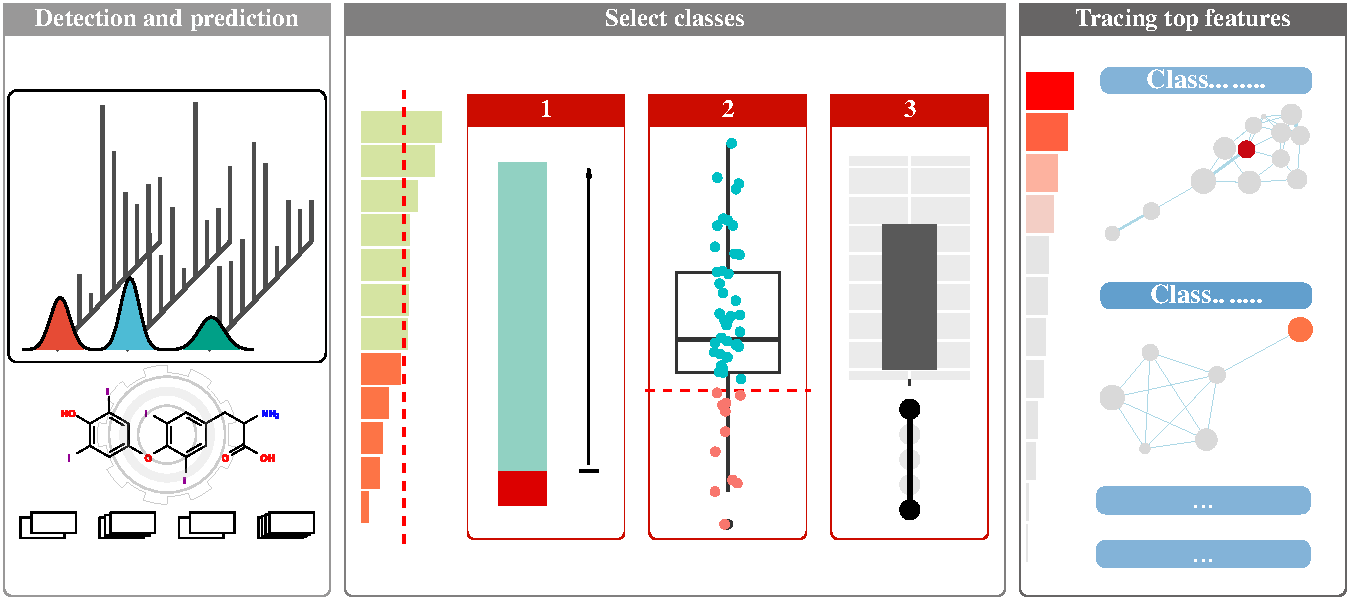
\includegraphics{tocg.pdf}

\textbf{Keywords:} Mass spectrometry, visualization, chemical classes,
identification, MCnebula

\hypertarget{introduction}{%
\subsection{Introduction}\label{introduction}}

Analyzing untargeted liquid chromatography/tandem mass spectrometry
(LC-MS/MS) dataset is complicated, due to the massive of data volume,
complexity of spectra and structural diversity of compounds. In the past
decades, a lot of researchers attempted to address the issues. Many
technical software or web-based interfaces were developed to provide a
one-stop bulk solution for data
analysis\textsuperscript{\protect\hyperlink{ref-2020p}{1}--\protect\hyperlink{ref-2016a}{4}}.
These solutions applied or suggested flexible mass spectra processing
tools or analogous
algorithms\textsuperscript{\protect\hyperlink{ref-2012d}{5}--\protect\hyperlink{ref-2010}{8}}.
To reduce false-positive and false-negative results, more algorithms
have been implemented for peak deconvolution, feature selection or
statistical
filtering\textsuperscript{\protect\hyperlink{ref-2017f}{9}--\protect\hyperlink{ref-2022b}{12}}.
Every feature corresponding to a compound within sample or parallel
samples was prevalently equipped with fragmentation spectra for
identification. In this context, researchers have to be confronted with
a problem: how to identify so many compounds accurately and quickly?

Until today, several strategies were developed for identifying compounds
with fragmentation spectra. \textbf{1)} Spectral library matching. A
number of public available databases were built to settle that via
achieving re-usability of reference fragmentation spectra, such as
MassBank, MassBank of North America (MoNA), Global Natural Products
Society molecular networking
(GNPS)\textsuperscript{\protect\hyperlink{ref-2016a}{4}}. In the
meanwhile, these fragmentation spectra are available via their web
servers, third-party platform (e.g.,
\href{http://prime.psc.riken.jp/compms/msdial/main.html\#MSP\%3E}{CompMass})
or specific tools
(MASST)\textsuperscript{\protect\hyperlink{ref-2020cm}{13}}. However,
compared with structure database (PubChem harbours over 100 million
records), spectral library is too small in size that limit the
application of mass spectrometry. To cross this barrier, \textbf{2)}
\emph{In silico} simulation by fragmentation spectra. \emph{In silico}
tools have been increasingly developed for simulating fragmentation
spectra\textsuperscript{\protect\hyperlink{ref-2010c}{14}--\protect\hyperlink{ref-2017aq}{17}}.
Some databases such as MoNA collated \emph{in silico} fragmentation
spectra and were available for
public\textsuperscript{\protect\hyperlink{ref-2013w}{18}}. \textbf{3)}
\emph{In silico} prediction with matching learning. At present, the
algorithms made machine training from reference mass dataset or
libraries, then `learned' how to predict chemical fingerprints or
principles so as to retrieve the correct structure from structure
database\textsuperscript{\protect\hyperlink{ref-2012ab}{19}--\protect\hyperlink{ref-2018ay}{21}}.

\emph{In silico} methods are developing quickly. Up to now, the
cutting-edge technology, called SIRIUS
4\textsuperscript{\protect\hyperlink{ref-duhrkop_sirius_2019}{22}},
integrated with many advanced algorithms of artificial intelligence, was
reported that its accuracy rate reached to 70\% while retrieving in
structure libraries. This method helps to identify metabolites beyond
the scope of spectral libraries. While \emph{in silico} tools boost
chemical identification, it is still lack of a proper framework that
could incorporate and leverage SIRIUS 4 into user-friendly way for
biological research, such as~biomarker discovery and pathway analysis of
mass spectral dataset. Compounds annotation and screening of biomarkers
manually are both time-consuming and the results are impressed by
subjective factors. Molecular networking is more and more popular due to
its visualization and data transparency. Molecular networking was a
spectral correlation and visualization method that can detect spectra
from related molecules (so-called spectral networks), even when the
spectra were not matched to any known
compounds\textsuperscript{\protect\hyperlink{ref-2016a}{4}}. Based on
the concept of molecular networking, we proposed an idea, clustering
features for visualization of chemical classification probably
contribute to the discovery of biomarkers and metabolic pathway
analysis.

The history of classification in chemistry dated back to the middle of
the last century. The Chemical Fragmentation Coding system was firstly
developed by Derwent World Patent Index (DWPI) in 1963. Until recent
years chemical classification like Gene Ontology
(GO)\textsuperscript{\protect\hyperlink{ref-2000g}{23}} which was
organized with taxonomy and ontology was proposed more
systematically\textsuperscript{\protect\hyperlink{ref-2016}{24}}.
ClassyFire is popular for compound annotation in LC-MS dataset analysis
due to its computation available and
systematicness\textsuperscript{\protect\hyperlink{ref-2019bt}{25}--\protect\hyperlink{ref-2019bq}{28}}.
The taxonomy and ontology is robust and useful for chemistry. For
example, a hierarchical classification-based method, called Qemistree,
was proposed to analyze mass spectrometry data by expressing molecular
relationships as a tree, which could be represented in the context of
sample metadata and chemical
ontologies\textsuperscript{\protect\hyperlink{ref-2021b}{29}}.

Untargeted metabolomics is a field of omics science that uses
cutting-edge analytical chemistry techniques and advanced computational
methods to characterize complex biochemical mixtures aimlessly.
LC­MS-based untargeted metabolomics is very popular due to its high
sensitivity, small sample volume and direct injection without separation
etc.\textsuperscript{\protect\hyperlink{ref-2016aq}{30}}. With the help
of statistical methodologies, researchers could screen and identify
more-informative disease biomarkers from thousands of LC-MS features, to
aid the design or development of improved treatments and to better
assess health
outcomes\textsuperscript{\protect\hyperlink{ref-2016ar}{31}}. . These
statistical approaches mainly involved classical statistic and
artificial intelligence models(e.g., random
forests)\textsuperscript{\protect\hyperlink{ref-2019bv}{32}}. Both
approaches were inevitable to introduce specific biases, owing to the
complexity of feature set or algorithmic
stability\textsuperscript{\protect\hyperlink{ref-2017i}{33}}.
Furthermore, analyzing at feature level was unable to profile systematic
effects on metabolites
unbiased\textsuperscript{\protect\hyperlink{ref-duhrkop_systematic_2021}{34}}.
In this view, analyzing at chemical classified level may be a better
settlement. However, it shouldn't be ignored that the differences of
metabolites at the same classified level. For example, small-molecules
belonging to `Indoles and derivatives' had structural dependent
affection on aryl hydrocarbon receptor
(AHR)\textsuperscript{\protect\hyperlink{ref-2019c}{35}}. Different
structural characteristics will lead to diverse activities. The
settlement for that is integrating both `feature' level statistic and
classified level assessment.

In addition to chemical classifying and statistical analysis, clustering
visualization was also a popular tool for untargeted mass spectrometry
data analysis. Over the last decade, Global Natural Products Social
Molecular Networking (GNPS) is more and more popular as a clustering
visualization tool based on MS dataset. GNPS applied molecular
networking connecting mass spectra of molecules based on the similarity
of their fragmentation
patterns\textsuperscript{\protect\hyperlink{ref-2012a}{36}}.
Unfortunately, molecular networking of GNPS mainly depend on on spectral
similarity instead of compounds structural or classified similarity. For
example, flavonoids consist of an aromatic ring joined to an oxygenated
heterocyclic ring linked to a phenyl group,which were expected to be
clustered together since its specific class and structural similarity.
However, , it was reported that some compounds belonging to flavonoids
happened to be absent from the cluster of other flavonoids compounds in
previous
research\textsuperscript{\protect\hyperlink{ref-duhrkop_systematic_2021}{34}}.
Thus, clustering visualization in a classified level is a better choice
for untargeted mass spectra dataset. Earlier in 2012, the concept of
molecular networking with visualization for mass data analysis was
proposed for the first
time\textsuperscript{\protect\hyperlink{ref-2012a}{36}} but \emph{in
silico} tools for predicting compound classification by fragmentation
spectra were not available at that time. Nowadays, with the development
of automatic classified \emph{in silico}
tools\textsuperscript{\protect\hyperlink{ref-2016}{24}}, it is time for
a revolution of the visualization strategy with higher confidence in
classified level.

For above consideration, we proposed a comprehensive framework, named
MCnebula, for untargeted LC-MS/MS dataset analysis. MCnebula integrated
a new abundance-based classes (ABC) selection algorithm for chemical
classes selection. The principle of ABC selection algorithm: (1) applied
an initial filtering to thousands of chemical classes based on the
predicted probability, (2)regarded all `features' as a whole, examined
the number and abundance of `features' of each chemical classification
(classification at different levels, classification of sub-structure and
dominant structure), and then selected representative classes, (3)these
chemical classes were followed by goodness assessment (about
identification of its classified compounds) and identicality assessment
(the extent to which these chemical classes are distinguished from each
other in the context of MS/MS spectra). The final chemical classes would
serve to the subsequent analysis: visualized as Child-Nebulae and focus
on these chemical classes / Nebulae for biomarker or chemistry
discovery. The top `features' based on statistical analysis could be set
as tracer to discover more homology compounds of chemical structure or
spectral similarity or chemical class. MCnebula can be used to explore
unknown compounds because of the annotation module and the cutting-edge
technology of SIRIUS
software\textsuperscript{\protect\hyperlink{ref-duhrkop_searching_2015}{20},\protect\hyperlink{ref-duhrkop_sirius_2019}{22},\protect\hyperlink{ref-duhrkop_systematic_2021}{34},\protect\hyperlink{ref-bocker_sirius_2009}{37}--\protect\hyperlink{ref-ludwig_database-independent_2020}{39}},
which exceeded the limitations of spectral library matching. MCnebula
was implemented in the R language and can be easily integrated into the
diverse biological analysis workflow of R. MCnebula (updated to
MCnebula2, which included more tools such as ABC selection algorithm,
Nebula visualization, statistical analysis, and output report etc.) was
written primarily in S4 system of object-oriented programming. It
allowed all data for one-button analysis from the beginning to the end,
which facilitated data processing. In addition to the basic function of
MCnebula), we provided an additional `exMCnebula2' package for
downstream analysis, which contained all the analysis tools used in this
study such as pathway enrichment analysis, heatmap clustering analysis,
spectral visualization analysis, chemical information query, etc.
Downstream analysis of untargeted LC/MS-MS is complex and varies from
data to data. The additional tools in exMCnebula2 package could provide
a prototype for the expanded application of MCnebula.

In this article, two datasets were applied in MCnebula in order to
demonstrate the broad utility of our method. One was a human-derived
serum dataset that correlated with mortality risk profiling of
staphylococcus aureus Bacteremia (SaB); the other was a plant-derived
herbal dataset that related to the traditional processing of herbal
medicine.

\hypertarget{experimental-section}{%
\subsection{Experimental section}\label{experimental-section}}

\hypertarget{mcnebula-algorithm}{%
\subsubsection{MCnebula algorithm}\label{mcnebula-algorithm}}

\textbf{Overall consideration} The analysis of untargeted LC-MS/MS
dataset generally begins with feature detection. Features are recognized
as ``peaks'' in MS\textsuperscript{1} (MASS level 1) data. Each feature
may represent a compound, and assigned with MS\textsuperscript{2} (MASS
level 2) spectra. The MS\textsuperscript{2} spectra was then used to
figure out the compound identity. The difficulty was mainly in
annotating these features to discover their compound identity and mining
out useful information for further biological research. In addition, the
untargeted LC-MS/MS dataset was generally a huge dataset, which leads to
time-consuming analysis of the whole process. Herein, a classified
visualization method, called MCnebula, was used for addressing these
issues.

The MCnebula package itself does not involve molecular formula
prediction, structure prediction or chemical prediction of compounds,
thus the accuracy of these parts was not considered. MCnebula achieved
downstream analysis by extracting the prediction data from SIRIUS
project. The core of MCnebula was chemical classes filtering algorithm,
which was called abundance-based classes (ABC) selection algorithm. To
explain the ABC selection algorithm in detail, we need to begin with
MS/MS spectral analysis and identify compounds.

\textbf{Chemical structure and formula.} The analysis of MS/MS spectrum
was a process of inference and prediction. For example, we speculated
the composition of elements based on the molecular weight combined with
the possible fragmentation pattern of MS/MS spectrum, we speculated the
potential molecular formula of a compound. Finally, we looked for the
exact compound from the compound structure database. Sometimes, this
process is full of uncertainty, because there were too many factors that
could affect the reliability of MS/MS data and the correctness of
inference. It can be assumed that there are complex candidates for the
potential chemical molecular formula, chemical structure and chemical
class behind MS/MS spectrum. Suppose we had these data of candidates
now, MCnebula could help extract these candidates and obtain the unique
molecular formula and chemical structure for each MS/MS spectrum based
on the highest score of chemical structure prediction; in this process,
like most algorithms, we can filter the prediction based on score.

\textbf{Establish reference upon top candidate} We predicted a potential
compound represented by LC-MS/MS spectrum, and obtained the candidates
of chemical molecular formula, structure and chemical class. These
candidates include both positive and negative results: for chemical
molecular formula and chemical structure, the positive prediction was
unique; for chemical class, multiple positive predictions that belonged
to various classification were involved. We did not know the exact
negative and positive modes. Normally, we ranked and filtered these data
by score. There were numerous scores, for isotopes, for mass error, for
structural similarity, for chemical classes and so on. Selection of
score for ranking candidates depended on the purpose of research. For
instance:

\begin{itemize}
\item
  To find out the chemical structure mostly be positive mode, ranking
  the candidates by structural score.
\item
  To determine whether a potential compound belongs to a certain
  chemical class, ranking the candidates by the classified score.
\end{itemize}

By functions in MCnebula of `filter\_formula()', `filter\_structure()'
or `filter\_ppcp()', the candidate with top score can be obtained.
However, for the three module (formula, structure, classes), sometimes
their top score candidates were not in line with each other. That was,
their top score towards different chemical molecular formulas. To find
out the corresponding data in other modules, `create\_reference()'
should be performed to establish the `specific candidate' as reference
for subsequent data integrating.

We obtained the unique chemical molecular formula and chemical structure
formula for reference by scoring and ranking. But for chemical classes,
such method was not enough.

\textbf{Chemical classification.} Chemical classification is a complex
system. Here, we only discuss the structure-based chemo taxonomy
system\textsuperscript{\protect\hyperlink{ref-2016}{24}}, because the
MS/MS spectrum is more indicative of the structure of compounds than
biological activity and other information.

According to the division of the overall structure and local structure
of compounds, we can call the structural characteristics as the dominant
structure and
substructure\textsuperscript{\protect\hyperlink{ref-2016}{24}}.
Correspondingly, in the chemical classification system, we can not only
classify compounds according to the dominant structure, but also
classify according to the substructure. The chemical classification
based on the dominant structure of compounds is easy to understand. For
example, we will classify Taxifolin as `Flavones', not `phenols',
although its local structure has a substructure of `phenol'. We hope to
classify a compound by its dominant structure rather than substructure,
because such classify is more concise and contains more information.
However, in the process of MS/MS spectral analysis, we sometimes can
only make chemical classification based on the substructure of
compounds, which may be due to: uncertainty in the process of structural
analysis; it may be an unknown compound; MS/MS spectral fragment
information is insufficient. In this case, it was necessary for us to
classify the compounds with the aid of substructure information,
otherwise we had no knowledge of the compounds for which we cannot
obtain dominant structure information.

We should also be clear about the complexity of another aspect of chemo
taxonomy, i.e., the hierarchy of classification. For example, `Flavones'
belongs to its superior, `Flavonoids'; its next higher level,
`Phynylpropanoids and polyketides'; the further upward classification is
`organic compounds'.

\textbf{ABC selection.} In the untargeted LC-MS/MS dataset, each feature
has a corresponding MS/MS spectrum, and there are thousands of features
in total. The ABC selection algorithm took all features as a whole,
examined the number and abundance of features of each chemical
classification (classification at different levels, classification of
substructure and dominant structure), and then selected representative
classes (mainly screening the classes according to the number or
abundance range of features) to serve the subsequent analysis (Fig.
\ref{fig:mech}).

\begin{figure}
\hypertarget{fig:mech}{%
\centering
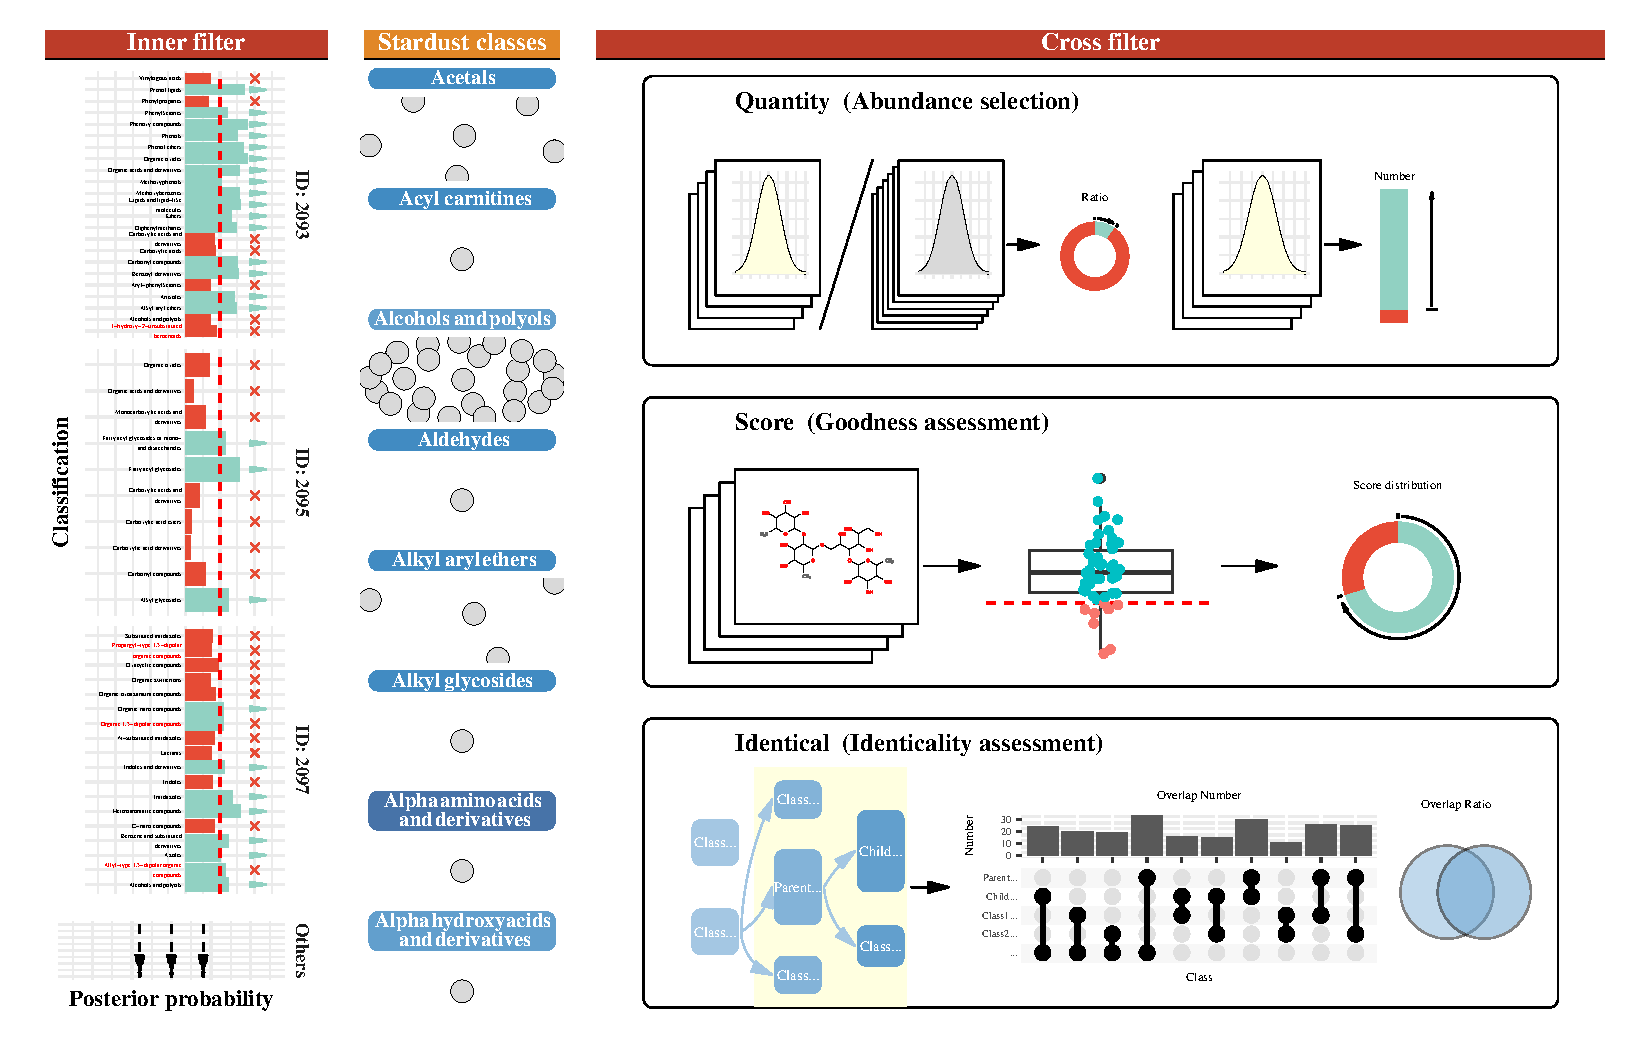
\includegraphics{fig1.mech.pdf}
\caption{\textbf{Mechanism for filtering chemical classes of MCnebula2.}
This figure illustrates how MCnebula2 filters chemical classes of
prediction from `features' to form a Nebula-Index to create
Child-Nebulae. The \textbf{Inner filter} filter out the chemical classes
by Regex match of names (names without without Arabic numerals) and set
threshold for value of posterior probability. To create \textbf{Stardust
Classes}, the previous filtered data is re-grouped according to chemical
classes instead of `features' ID. The \textbf{Cross filter} conduct
further filtering of chemical classes via combining Stardust Classes and
`features' annotation data. The details of Cross filter was described in
MCnebula2 Algorithm section in article.}\label{fig:mech}
}
\end{figure}

\begin{itemize}
\item
  Create Stardust Classes (Inner filter). The posterior probability of
  classification prediction (PPCP) data belonged to each `feature'. When
  performing the filtering, only simple threshold conditions or absolute
  conditions were set to filter the chemical classes; there was no
  crossover between the different attributes and no crossover between
  the `features'. Therefore, we considered this as `inner' filtering.
\item
  Cross filter Stardust Classes. The data of the chemical classes and
  their classified `features', i.e.~Stardust Classes data, were combined
  and then grouped upon the chemical classes. After grouping, each
  chemical class had a certain quantity of `features'. When filtering,
  statistics may be performed on `features' data within a group;
  statistics may be performed on these data in conjunction with
  `features annotation' data; and statistics may be performed to compare
  groups with each other. As its crossover of attributes for filtering,
  we consider this as `cross' filtering. (See details in next subsection
  about Cross filter Stardust Classes.)
\end{itemize}

Whether it is all filtered by the algorithm provided by MCnebula
function or custom filtered for some chemical classes, we now have a
data called Nebula-Index. This data records a number of chemical classes
and the `features' attributed to them. The subsequent analysis process
or visualization will be based on it. Each chemical class is considered
as a `nebula' and its classified `features' are the components of these
`nebulae'. In the visualization, these `nebulae' will be visualized as
networks. Formally, we call these `nebulae' formed on the basis of
Nebula-Index data as Child-Nebulae. In comparison, when we put all the
`features' together to form a large network, then this `nebula' is
called Parent-Nebula.

\textbf{Details of Cross filter Stardust Classes}. This method was an
integration of the three modules below (Fig. \ref{fig:mech}):

\emph{Cross filter by `quantity'} (abundance selection). Set `features'
quantity limitation for each group (each group, i.e.~a chemical class
with its classified `features'). The groups with too many `features' or
too few `features' would be filtered out. This means the chemical class
would be filtered out. These thresholds are about:

\begin{itemize}
\tightlist
\item
  Minimum quantity: the `features' within the group.
\item
  Maximum proportion: the `features' quantity within the group versus
  all `features' (unique) quantity of all groups.
\end{itemize}

The purpose of this step is to filter out the chemical classes that have
too large or too subtle a conceptual scope. For example, `Organic
compounds', which covers almost all compounds that can be detected in
metabolomics data, is too large in scope to be of any help to our
biological research. The setting of parameters is not absolute, and
there is no optimal solution. Users can draw up thresholds according to
the necessity of the study.

\emph{Cross filter by `score'} (Goodness assessment). This step
associate Stardust Classes data with `features' annotation data. For
each group, the Goodness assessment is performed for each target
attribute (continuous attribute, generally be a scoring attribute of
compound identification, such as `Tanimoto similarity'). If the group
met all the expected Goodness, the chemical class would be retained;
otherwise, the chemical class would be filtered out. The Goodness
(\(G\)) related with the `features' within the group:

\begin{itemize}
\item
  \(n\): the quantity of `features' of which target attributes satisfied
  with the cut-off.
\item
  \(N\): the quantity of all `features'.
\end{itemize}

The Goodness: \(G = n/N\).

The assessment of Goodness is related to the parameters of `tolerance'
and `cutoff':

\begin{itemize}
\tightlist
\item
  Expected Goodness, i.e.~value of `tolerance'.
\item
  Actual Goodness, related to parameter `cutoff'. \(G = n/N\).
\end{itemize}

Goodness assessment can be given to plural target attributes. Note that
the chemical class would be retained only if it passed the Goodness
assessment of all target attributes. The main purpose of this step is to
filter out those chemical classes with too many `features' of low
structural identification.

\emph{Cross filter by `identical'} (identicality assessment). A
similarity assessment of chemical classes. Set a hierarchical range for
chemical classification and let groups within this range be compared for
similarity to each other. For two groups, if the classified `features'
are almost identical to each other, the chemical class represented by
one of the groups would be excluded. The assessment of identical degree
of two groups (A and B):

\begin{itemize}
\tightlist
\item
  \(x\): ratio of the classified `features' of A belonging to B
\item
  \(y\): ratio of the classified `features' of B belonging to A
\item
  \(i\): value of parameter `identical\_factor'
\end{itemize}

If \(x > i\) and \(y > i\), the two groups would be considered as
identical. Then the group with fewer `features' would be discarded. The
purpose of this step is to filter out classes that may incorporate each
other and are similar in scope. The \emph{in silico} prediection
approach may not be able to distinguish which class the potential
compound belongs to from the LC-MS/MS spectra.

\textbf{Network graph presentation} As mentioned above, `features' and
their annotations were integrated as Nebulae according to the
Nebula-Index. These Nebulae were network-type graph data. The `features'
annotation data contains top candidate of chemical formula and structure
(obtained with the MCnebula function `filter\_*()'). The MS/MS spectral
similarity (dot product) of the `features' was calculated and used to
form the edge data for the network graph.

\textbf{Visualization system} MCnebula used a number of existing R
packages to integrate and reformat data. In particular, the network
graph data was equipped with `ggplot2' package for visualization. The
ggplot2 package is known for its elaborate and aesthetic mapping
characteristics. We designed the `ggset' data class to store pre-defined
ggplot2 plotting functions and parameters for visualizing Nebulae. This
allows users to completely customize the visualization to suit their
needs or the needs of the publisher. Its flexibility depends on the
user's understanding and proficiency of the `ggplot2' package. If users
are not experienced in using the `ggplot2' package, he should just
follow the preset package for visualization.

\textbf{Statistic analysis} MCnebula integrated the functions (mainly
for: `limma::makeContrasts', `limma::lmFit', `limma::lmFit',
`limma::eBayes') of the `limma' package for differential expression
analysis (analysis of RNA-sequence and microarray) and packaged them for
differential analysis of metabolomics
data\textsuperscript{\protect\hyperlink{ref-gentleman_limma_2005-1}{40}}.
The gene expression matrix and the feature quantification matrix of
LC-MS are similar, both of which have corresponding explanatory
variables (sample information) and dependent variables (gene expression
values or feature quantification values), except that one represents the
level of gene expression and the other the level of metabolite. We
normalized the peak area levels of the features and transformed (log2)
them, used the metadata information of the samples to create the design
matrix and the contrast
matrix\textsuperscript{\protect\hyperlink{ref-gentleman_limma_2005-1}{40}};
thus even if the data itself is not gene related, it can be performed
differential analysis using the tools of the `limma' package. The
`limma' is a powerful package for differential analysis using linear
models that can handle not only simple experimental designs in which the
explanatory variables are factors (e.g., Control group versus Model
group), but also complex experimental designs in which the explanatory
variables are covariates (e.g., groups containing time series). However,
our packaged method was only appropriate to experimental designs in
which explanatory variables are factorial variables and the design
matrix without intercept (code: `model.matrix(\textasciitilde{} 0 +
group)')\textsuperscript{\protect\hyperlink{ref-law_guide_2020}{41}}.
Because of its simple applicability, we called it `binary comparison'.
Our evaluation section does not cover its evaluation (as it is not the
main part of this study), but we used it in two demo datasets and
validated them to some extent: in the serum dataset, we compared our
obtained top `features' with that of Wozniak et
al.\textsuperscript{\protect\hyperlink{ref-2020s}{42}}; in the herbal
dataset, we traced the obtained top `features' to the EIC plot.

\textbf{Data structure} MCnebula was written mainly in R S4 system of
object-oriented programming. When we analyzed data with MCnebula, all
data (whether `features' annotation data or visualization data) was
stored in a one object (class `mcnebula'). This reduced the difficulty
of using the MCnebula package, and made the data easy to manage and the
analysis easy to repeat.

\textbf{Report system} MCnebula integrated a reporting system that
allows the analysis process to be output as a PDF document or in other
formats. The reporting system was based on the data class `report',
which could stores each step of the analysis as a section and could be
flexibly modified according to the user's needs. In addition, the
reporting system can be used to generate reports even if the analysis is
completely irrelevant to MCnebula package. The reporting system was
associated with the `rmarkdown' R
package\textsuperscript{\protect\hyperlink{ref-xie_r_2020}{43}}.

\textbf{Code Compatibility} MCnebula conducted downstream analysis by
extracting the data from the already computed SIRIUS project. The SIRIUS
project is the main source of data for MCnebula 2. The SIRIUS software
is still being updated and improved. In fact, from SIRIUS version 4 to
version 5 (\url{https://github.com/boecker-lab/sirius}), the data
structure and attributes name in the project directory have changed. In
order that the functionality of MCnebula is not invalidated due to
versioning issues, its application program interface (API) for the
SIRIUS project has been designed to be flexible. MCnebula is able to
perform data extraction for different SIRIUS versions.

\hypertarget{mcnebula-evaluation}{%
\subsubsection{MCnebula evaluation}\label{mcnebula-evaluation}}

\textbf{Spectra dataset for evaluation.} The spectra collection (in
positive ion mode, for more spectra data) of GNPS MS/MS library was used
for evaluation (.msp file)
(\url{http://prime.psc.riken.jp/compms/msdial/main.html\#MSP}). As
Fragmentation spectra in reference library generally possess high
quality, and while used for evaluation of library match, it may cause
overfitting. To address the issue, refer to
ref.\textsuperscript{\protect\hyperlink{ref-2021}{44}}, we added `noise'
into these MS/MS spectra. In brief, the `noise' involves mass shift,
intensity shift, and the inserted noise peak; of note, the magnitude
factors for these shift were drawn randomly from function of normal
distribution. Overall, we simulated two model of `noise' (medium noise
and high noise). The `noise' simulation was achieved in custom R script.
These algorithms and parameters were parallel to the
reference\textsuperscript{\protect\hyperlink{ref-2021}{44}}. We assigned
these datasets as origin dataset, medium noise dataset and high noise
dataset. The details of simulation of noise were as following:

\begin{itemize}
\item
  A global mass shift was simulated by drawing a random number
  \(\delta^{*}\) from \(N\left( 0,\sigma_{mb}^{2} \right)\) (Normal
  distribution) and then shifting every peak mass \(m\) by
  \(\delta^{*}m\). The standard deviation \(\sigma_{mb}\) was chosen as
  \(\sigma_{mb} = (10/3) \times 10^{- 6}\) (medium noise) or
  \(\sigma_{mb} = (15/3) \times 10^{- 6}\) (high noise), so that the
  \(3\sigma_{mb}\) interval represents a 10-ppm shift for medium noise
  and a 15-ppm shift for high noise.
\item
  Individual mass deviations was simulated by drawing, for each peak
  with mass \(m\) individually, a random number \(\delta\) from
  \(N\left( 0,\sigma_{md}^{2} \right)\) and shifting the peak by
  \(\delta m\). The standard deviation \(\sigma_{md}\) was chosen so
  that the \(3\sigma_{md}\) interval represents a 10-ppm shift for
  medium noise and a 20-ppm shift for high noise.
\item
  Intensity variations were simulated in the spectrum. Each peak
  intensity was multiplied by an individual random number \(\epsilon\)
  drawn from \(N\left( 1,\sigma_{id}^{2} \right)\). Variance was chosen
  as \(\sigma_{id}^{2} = 1\) for medium noise and
  \(\sigma_{id}^{2} = 2\) for high noise. 0.03 times the maximum peak
  intensity of the spectrum was subtracted from each peak intensity. If
  a peak intensity fell below the threshold of one thousands of the
  maximum intensity in the spectrum, the peak was discarded.
\item
  Additional `noise peaks' were added to the spectrum. In processing of
  origin dataset, a pool of `noise peaks' was gathered from the
  fragmentation spectra, using all peaks that did not have a molecular
  sub-formula decomposition of the known molecular formula of the
  precursor. For each spectrum, \(\alpha n\) of these `noise peaks' were
  added to the spectrum, where \(n\) is the number of peaks in the
  spectrum and \(\alpha = 0.2\) for medium noise and \(\alpha = 0.4\)
  for high noise. Intensities of `noise peaks' were adjusted for maximum
  peak intensities in the contributing and receiving spectrum. `Noise
  peaks' were randomly drew from the pool of `noise peaks' and added to
  the spectrum.
\end{itemize}

For another issue, the spectra collection did not possess isotopes
pattern. In real LC-MS processing (feature detection), isotope peaks
were grouped and merged, which favorable for SIRIUS to detect some
specific
element\textsuperscript{\protect\hyperlink{ref-bocker_sirius_2009}{37}}.
To simulate isotopes pattern, we used function of `get.isotopes.pattern'
within `rcdk' R package to get isotope mass and its
abundance\textsuperscript{\protect\hyperlink{ref-2007j}{45}}.
Furthermore, these mass were considered for the adduct type to increase
or decrease exact mass. For the `intensity' of these isotope pattern, we
simulated as relative intensity, i.e., the abundance of isotopes
multiply by 100 by value. These `isotope peaks' were merged into
MS\textsuperscript{1} list of its compounds. All the spectra collections
were formatted to fit with input of MCnebula workflow or benchmark
method (.mgf file and feature quantified table .csv).

\textbf{Evaluation method.} The three simulated data were all run with
MCnebula workflow and benchmark method. While these data were put into
SIRIUS 4 command-line interface (CLI) (version 4.9.12) for computation,
the MS/MS spectra with empty fragmentation peak were auto-filtered. In
addition, to reduce computation time, the compounds with over 800 m/z
precursor were filtered out manually. These filtered out compounds were
excluded from ultimate accuracy assessment. There were 8782 MS/MS
spectra within the raw collection, and after filtered or excluded,
totally 7524 compounds for ultimate evaluation.

The assessment of classified accuracy was conducted with the help of
ClassyFire\textsuperscript{\protect\hyperlink{ref-2016}{24}}. In detail,
we traversed the raw .msp spectra file to collate metadata of these
compounds, involving structure annotation. The International Chemical
Identifier Key (InChIKey) of these compounds were available for
ClassyFire database retrieve. However, since ClassyFire only support
those chemical identity of which structure have been classified in its
server previously, we noticed all the InChIKeys were vetoed. To address
that, we employed first hash block of these InChIKeys (InChIKey planar,
represent molecular skeleton) to touch PubChem application programming
interface (API)
(\url{https://pubchemdocs.ncbi.nlm.nih.gov/pug-rest})\textsuperscript{\protect\hyperlink{ref-2022ak}{46}}.
Accordingly, we got all the possibly InChIKeys of isomerism (stereo,
isotopic
substitution)\textsuperscript{\protect\hyperlink{ref-2012e}{47}}. The
classification of small molecules depends on its molecular skeleton
hence these chemical identities possess the same InChIKey planar are
identical in classification. We pushed the obtained InChIKey list to
ClassyFire to obtain classification. In R script, once any InChIKey of
isomerism meet the classified data in database, the acquisition status
for this molecular skeleton was turned off. In the end, all these
chemical annotation were collated, integrated and assigned as standard
reference.

The discrepancies between the MCnebula and benchmark methods in terms of
algorithm and classified results disallow them to be evaluated at
completely the same level. We evaluated both methods respectively. For
MCnebula, before assess the accuracy, we interrogated the obtained
classes generated from pre-analysis of the origin dataset. The classes
over in half were classified based on sub-structural class, such as
`Organic carbonic acids and derivatives', `Hydroxy acids and
derivatives'. These classes were small in structural size and were
chemical function group within compounds. The principle of ClassyFire is
selecting the most dominant structural class of compounds to
substitute\textsuperscript{\protect\hyperlink{ref-2016}{24}}. But, in
perspective of drug discovery, structure determines potency; many
pharmacological action possibly depends on these sub-structure. To
locate more universality among features, in algorithm, we reserved these
classes in results. Sub-structural classify for benchmark method not
available, hence we neglected these classes in evaluation. The rest
classes, nevertheless, still possibly be sub-structural class while meet
some compounds. We assigned three levels for evaluation, i.e., `True',
`Latent', `False'. The `True' indicated the classified classes were in
line with that of ClassyFire. The `Latent' indicated the classified
classes were not in line with that of ClassyFire, but their parent
classes of `class' level were in line with that of ClassyFire. The
`False' indicated the classified classes were completely inconsistent
with that of ClassyFire.

To assess the identification of classes or structures, the results were
merge with standard reference by InChIKey planar. For assessment of
identification of chemical structure, once the identified chemical
structure was in line with or chemical structure (match by InChIKey
planar), we assigned it as `true'. Indeed, such evaluation neglect
stereochemistry.

\hypertarget{serum-dataset}{%
\subsubsection{Serum dataset}\label{serum-dataset}}

We re-analyzed 245 LC-MS/MS data (.mzML) from MASSIVE (id no.
MSV000083593) (blanks, controls and
samples)\textsuperscript{\protect\hyperlink{ref-2020s}{42}}. MZmine2
(version 2.53) was performed for feature detection. The detection
workflow mainly involves \textbf{1)} Automated Data Analysis Pipeline
(ADAP) for peak detection and
deconvolution\textsuperscript{\protect\hyperlink{ref-2017f}{9}},
\textbf{2)} isotopes peak finder, \textbf{4)} parallel samples join
alignment, \textbf{5)} gap filling algorithm. While we exported MS/MS
spectra (.mgf) for SIRIUS 4 software computation, spectra were merged
across samples into one fragmentation list with 30\% Peak Count
threshold filtering. The feature detection workflow was referred to FBMN
preprocessing and SIRIUS computational prerequisites. The output .mgf
was run with SIRIUS 4 software (version 4.9.12) for computation with
SIRIUS\textsuperscript{\protect\hyperlink{ref-duhrkop_sirius_2019}{22}},
ZODIAC\textsuperscript{\protect\hyperlink{ref-ludwig_database-independent_2020}{39}},
CSI:fingerID\textsuperscript{\protect\hyperlink{ref-duhrkop_searching_2015}{20}},
CANOPUS\textsuperscript{\protect\hyperlink{ref-duhrkop_systematic_2021}{34}}.
In particular, SIRIUS was customized set to detect Iodine element while
predicting formula. MCnebula package were used for subsequent data
analysis. All subsequent analysis have been organized into concise code
and exported as reports (see section of Data and code availability).

Kyoto Encyclopedia of Genes and Genomes (KEGG) metabolic pathway
enrichment analysis was performed with `Lysophosphatidylcholines' (LPCs)
and `Bile acids, alcohols and derivatives' (BAs), respectively. We used
the identified InChIKey planar of structures to hit compounds in
metabolic pathway. In detail, firstly, in order to avoid the identified
structural deviations due to stereoisomerism, the InChIKey planar was
used to obtain all possible InChIKeys via PubChem API. In this step,
PubChem CID of those compounds were also obtained. The R package of
MetaboAnalystR was used for converting PubChem CID to KEGG
ID\textsuperscript{\protect\hyperlink{ref-2020cx}{48}}. Many compounds
were not related to metabolic pathway so those were filtered out. The R
package of FELLA was used for KEGG enrichment with `pagerank'
algorithm\textsuperscript{\protect\hyperlink{ref-2018bj}{49}}. The above
methods have been integrated as functions to interface with the MCnebula
workflow. These functions are available in the `exMCnebula2' package.

\hypertarget{herbal-dataset}{%
\subsubsection{Herbal dataset}\label{herbal-dataset}}

\textbf{Material and processing.} \emph{E. ulmoides} dried bark was
obtained from company of ZheJiang ZuoLi Chinese Medical Pieces LTD.
Raw-Eucommia and Pro-Eucommia were prepared as followed: (1)
Raw-Eucommia: The shreds or blocks of \emph{E. ulmoides} dried bark were
took, powdered and passed through 80-mesh sieves for further process.
(2) Pro-Eucommia: The shreds or blocks of \emph{E. ulmoides} dried bark
were sprayed with saline water (the amount of salt is 2\% of \emph{E.
ulmoides}, add 10 fold of water to dissolve), and smothered in airtight
for 30 min. Then, the barks were dried in oven at 60 °C, followed by
baking at 140 °C for 60 min. Finally, the baked barks were powdered and
passed through 80-mesh sieves for further process.

\textbf{Sample preparation.} 2 g of Raw-Eucommia powder and Pro-Eucommia
powder were weighed, respectively, added 50 ml of methanol/water (1:1,
v/v) followed by ultrasonic (20 kHz for 40 min). After ultrasonic, the
mixture was filtered to obtain filtrate and residue. The residue was
added with 50 ml of methanol/water (1:1, v/v) and extracted with
ultrasonic (40 kHz, 250 W for 20 min) again. The mixture was filtered.
Then, the filtrate of the two extracts was combined, the solvent was
evaporated. Methanol/water (1:1, v/v) was added to redissolve the
extract and the volume was fixed to 5 ml. Finally, the supernatant was
obtained by centrifugation (12,000 r.p.m. for 10 min) for further LC−MS
analysis.

\textbf{LC-MS experiments.} LC−MS analysis was performed using a Dionex
Ultimate 3000 UHPLC system (Dionex, Germany) coupled with a
high-resolution Fourier-transform mass spectrometer (Orbitrap Elite,
Thermo Fisher Scientific, Germany) using a Waters Acquity HSS T3 column
(1.8 \(mu\)m, 100 mm \(\times\) 2.1 mm, Waters Corporation, Milford, MA,
USA). Solvent A, formic acid/water (0.1:99, v/v), and solvent B, formic
acid/acetonitrile (0.1:99, v/v), were used as the mobile phase. The
gradient profile for separation was as follows: 2\% of solvent B at
0min, 5\% of solvent B at 2 min, 15\% of solvent B at 10 min, 25\% of
solvent B at 15 min, 50\% of solvent B at 18 min, 100\% of solvent B at
23 min, 2\% of solvent B at 25 min, and 2\% of solvent B at 30 min. The
flow rate was 0.3 ml/min. The column temperature was set at 40°C. Mass
spectrometric analysis was performed using an Orbitrap Elite instrument
equipped with an ESI source (Thermo FisherScientific, Germany) that
operated in the negative ionization mode. The ESI source was operated at
50 °C with a capillary temperature of 275 °C, an ionization voltage of
3.5 kV, and a sheath gas flow rate of 35 L/min. The survey scans were
conducted in the Orbitrap mass analyzer operating at a 120,000 (full
width at half-maximum) resolving power. A mass range of 100−1500 m/z and
a normalized collision energy of 30 eV were used for survey scans. The
analysis method was set to analyze the top 10 most intense ions from the
survey scan, and a dynamic exclusion was enabled for 15 s.

\textbf{MCnebula Workflow.} E.ulmoides dataset was preprocessed with
MZmine2 for feature detection, followed by SIRIUS software computation.
The subsequent analysis was similar to serum metabolic dataset and also
been organized as a report (see section of Data and code availability).

\hypertarget{data-processing}{%
\subsubsection{Data processing}\label{data-processing}}

Raw data (.raw) were converted to m/z extensible markup language (mzML,
i.e., .mzml format data) in centroid mode using MSConvert
ProteoWizard\textsuperscript{\protect\hyperlink{ref-2012d}{5}}. The
.mzml files were processed with MZmine2 (v.2.53) and followed by SIRIUS
4 in Pop!-OS (Ubuntu) 22.04 LTS 64-bits workstation (Intel Core
i9-10900X, 3.70GHz \(\times\) 20, 125.5 Gb of
RAM)\textsuperscript{\protect\hyperlink{ref-2010}{8}}. MCnebula
(MCnebula2) and other R packages were executed in Pop!\_OS (Ubuntu)
22.04 LTS 64-bits PC (Intel Core i7-1065G7, 1.3 GHz \(\times\) 8, 16 Gb
of RAM).

\hypertarget{data-and-code-availability}{%
\subsubsection{Data and code
availability}\label{data-and-code-availability}}

The source code of MCnebula was available at
\url{https://github.com/Cao-lab-zcmu/MCnebula}. The source code of
exMCnebula2 was available at
\url{https://github.com/Cao-lab-zcmu/exMCnebula2}. The code for all the
analysis in this study can be found in the internal data directory
(`inst/extdata/') of the `exMCnebula2' package. In addition, .mgf files
(msms spectra) and .csv files (feature quantification) and SIRIUS output
files (use MCnebula function to filter and compress tens of GB of data
to just a few tens of MB) and analysis report of serum and herbal
dataset were compressed and stored in the exMCnebula2 package. By
downloading and installing MCnebula package and exMCnebula2 package, all
the analyses of this study can be reproduced by executing R codes.

The serum dataset were available at MassIVE web service (id no.
\href{https://massive.ucsd.edu/ProteoSAFe/QueryMSV?id=MSV000079949}{MSV000083593}).
The submission job in GNPS of evaluation dataset are available: 1)
original dataset: FBMN:
\url{https://gnps.ucsd.edu/ProteoSAFe/status.jsp?task=05f492249df5413ba72a1def76ca973d}.
MolnetEnhancer:
\url{https://gnps.ucsd.edu/ProteoSAFe/status.jsp?task=9d9c7f83fa2046c2bf615a3dbe35ca62};
2) medium noise dataset: FBMN:
\url{https://gnps.ucsd.edu/ProteoSAFe/status.jsp?task=c65abe76cd9846c99f1ae47ddbd34927};
MolnetEnhancer:
\url{https://gnps.ucsd.edu/ProteoSAFe/status.jsp?task=7cc8b5a2476f4d4e90256ec0a0f94ca7};
3) high noise dataset: FBMN:
\url{https://gnps.ucsd.edu/ProteoSAFe/status.jsp?task=62b25cf2dcf041d3a8b5593fdbf5ac5e};
MolnetEnhancer:
\url{https://gnps.ucsd.edu/ProteoSAFe/status.jsp?task=f6d08a335e814c5eac7c97598b26fb80}.

\hypertarget{results-and-discussion}{%
\subsection{Results and discussion}\label{results-and-discussion}}

\hypertarget{results}{%
\subsubsection{Results}\label{results}}

\hypertarget{overview}{%
\paragraph{Overview}\label{overview}}

The MCnebula workflow was dedicated to analyzing LC-MS/MS datasets from
the beginning, i.e.~starting from the raw data obtained from the sample
and going through the various stages of analysis to obtain a complete
analysis report (Fig. \ref{fig:data_stream}). The analysis process
followed the general MCnebula analysis templates, from filtering
candidates of chemical formula, structural formulae, chemical classes,
to creating visual Nebulae; it also allowed for custom advanced
analysis, with the help of chemical class focused Nebulae, to perform
statistic analysis, features selection, focus on critical metabolites
(compounds) and their structural characteristics, pathway enrichment,
querying compound synonyms, etc. We evaluated workflow of MCnebula in
function with other popular public available methods. In terms of the
evaluation of our chosen indicators which cover identification,
classifying, etc., MCnebula has a wider scope of applicability. (Tab.
S1)

\begin{figure}
\hypertarget{fig:data_stream}{%
\centering
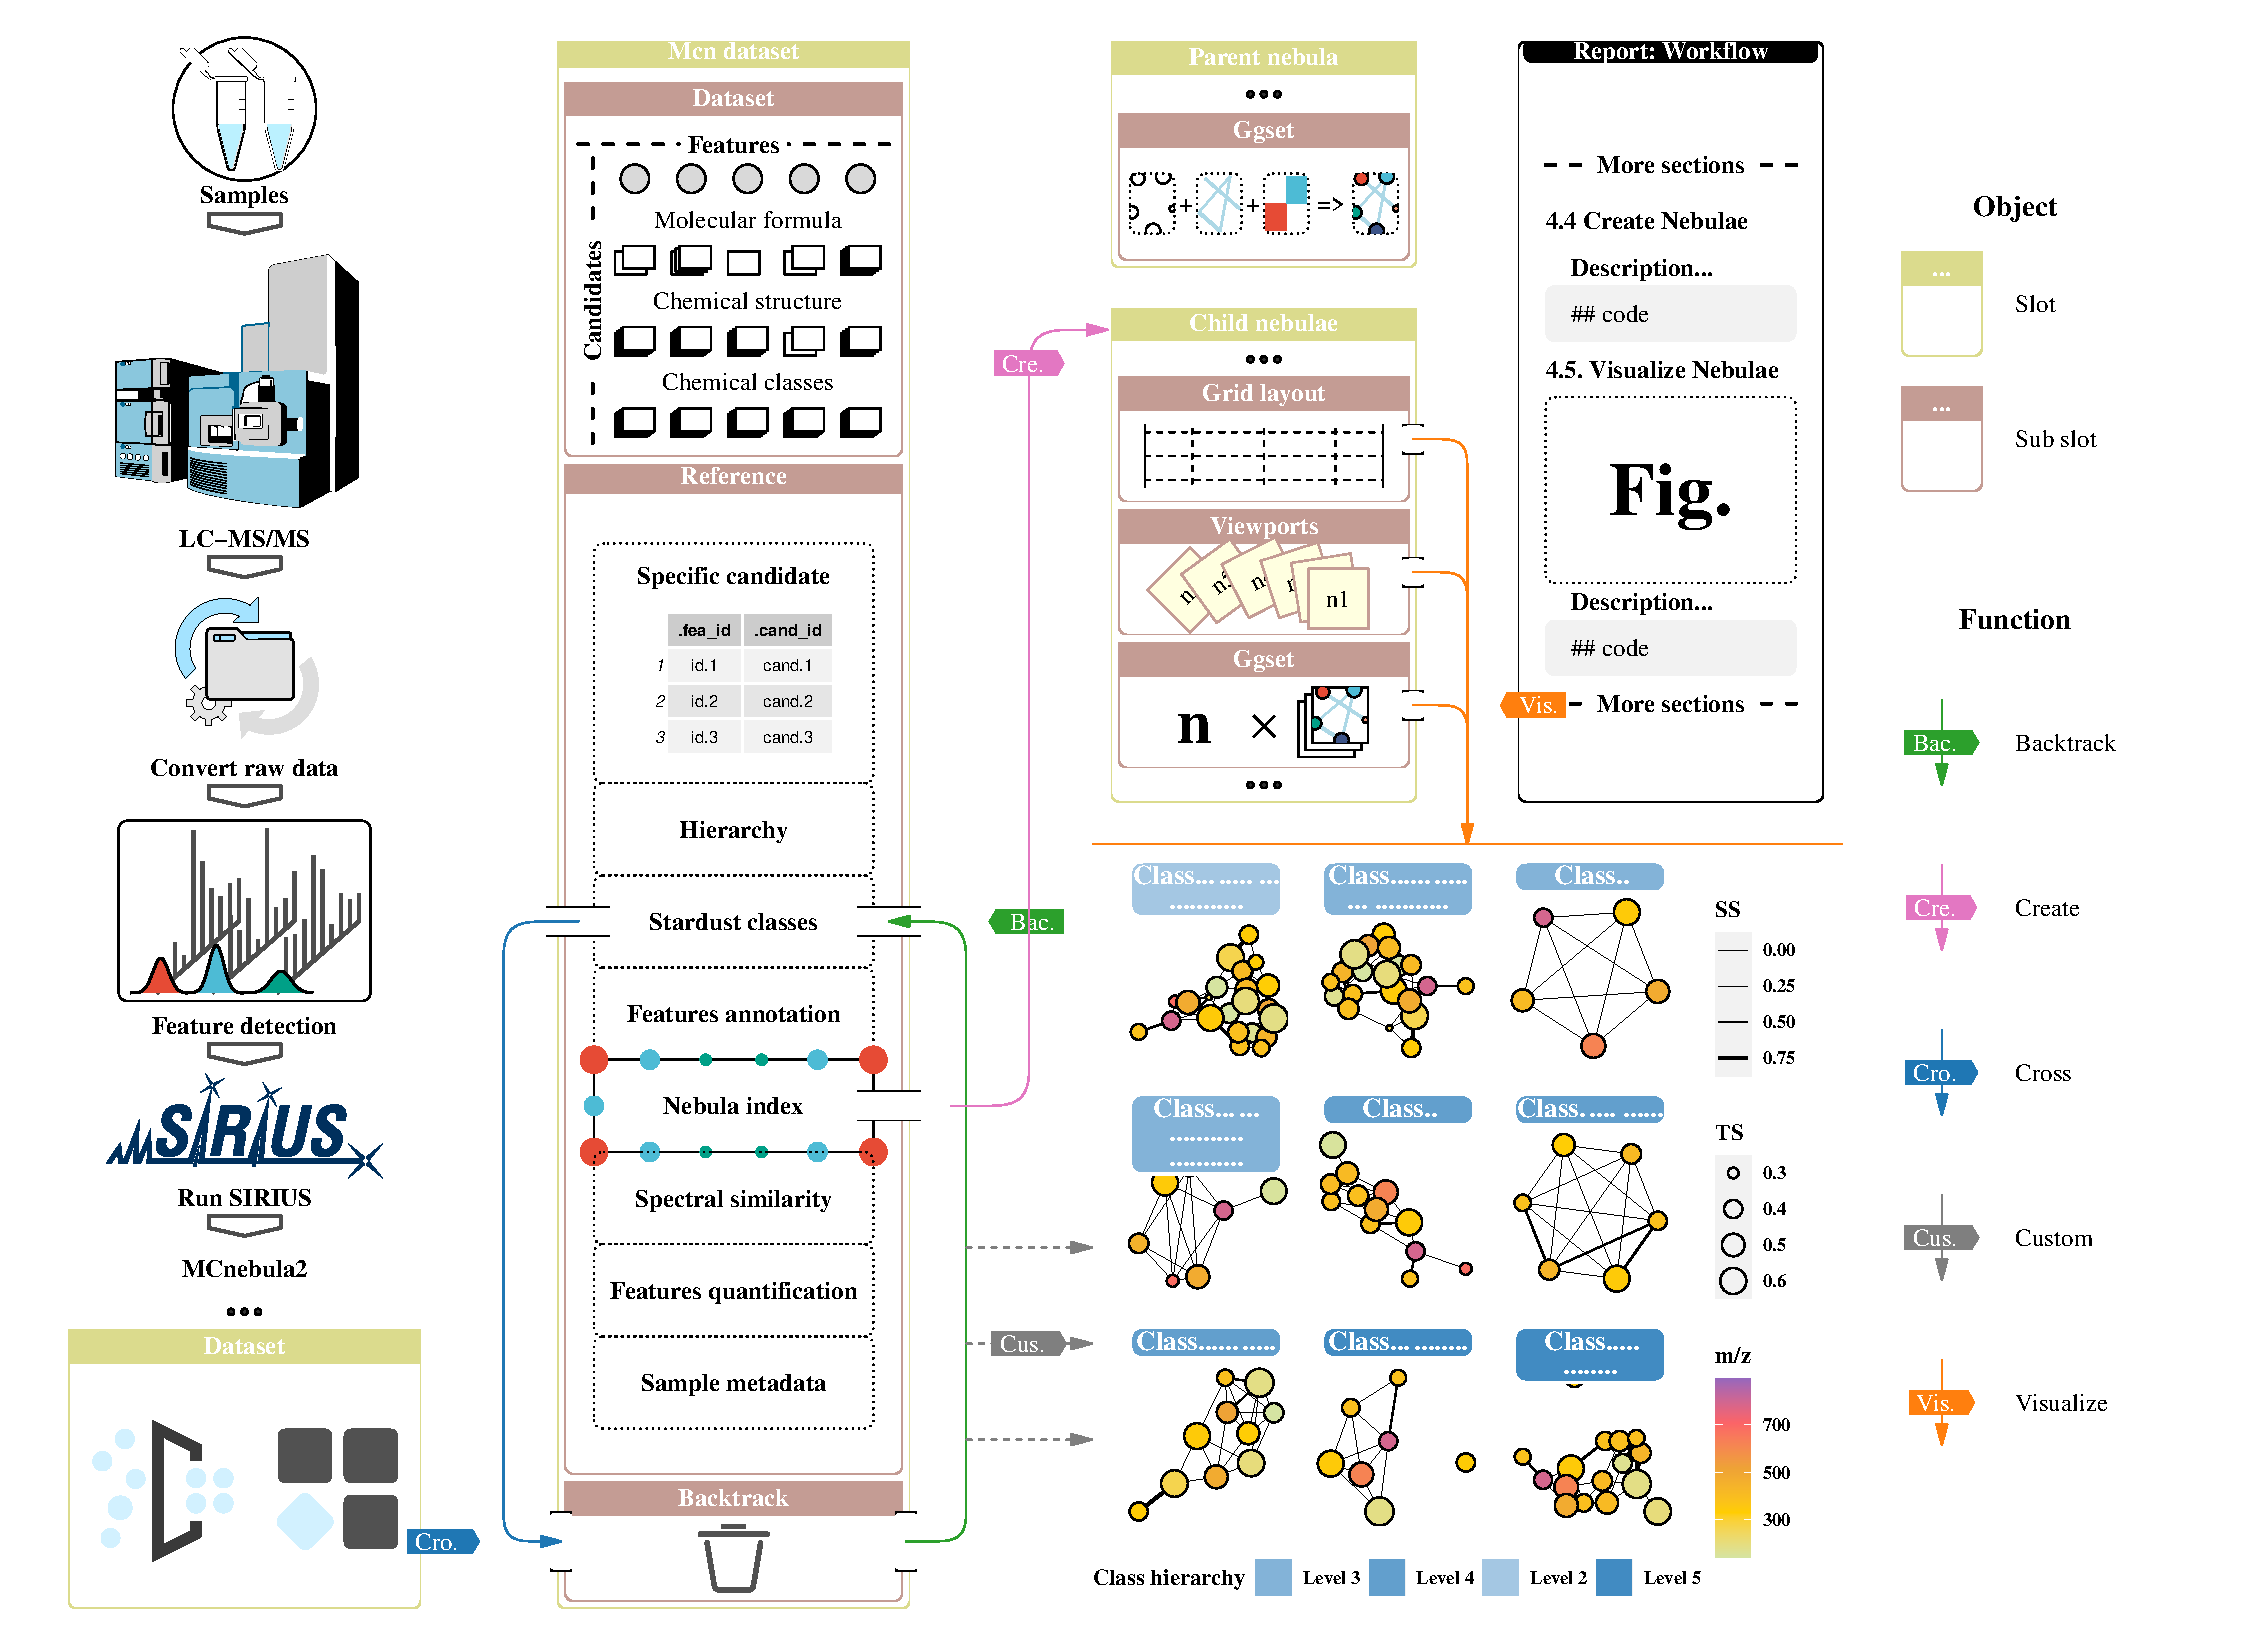
\includegraphics{fig2.data_stream.pdf}
\caption{\textbf{Data stream of MCnebula workflow.} The MCnebula
workflow can be divided into two parts, depending on the platform on
which the data presents. The first is the part beyond R (before
MCnebula2): from the \textbf{Samples} to \textbf{LC-MS/MS} to obtain the
raw data; the stage of \textbf{Convert raw data} is implemented using
the popular MSconvert tool derived from Proteowizard; for
\textbf{Feature detection}, users can implement it with any LC-MS
processing tool, such as MZmine, XCMS, OpenMS, etc.; then .mgf or other
file format of MS/MS spectra is imported into SIRIUS for computations.
The part inside R, MCnebula2 implements integrating data and creating
Nebulae within `mcnebula' object (see section of MCnebula2 algorithm in
article for details).}\label{fig:data_stream}
}
\end{figure}

\hypertarget{method-evaluation}{%
\paragraph{Method evaluation}\label{method-evaluation}}

\textbf{Classified accuracy.} We used a public available reference
spectral library to assess the accuracy of classifying by MCnebula. The
direct use of such a reference spectral library may lead to over-fitting
during the evaluation. We have taken the approach of simulating noise to
eliminate this consequence. Simulating noise, i.e., adding invalid noisy
data to the reference spectrum or numerically shifting the existing
data, also simulates data acquisition similar to a real scenario: due to
the different acquisition conditions, the spectral data in the real case
will be more noisy compared to the reference spectrum. By adding noise
to the reference spectral library, we now have three datasets for
evaluation (origin, medium noise and high noise dataset) (commonly 7524
compounds (spectra)). All three datasets were analyzed using MCnebula.
Due to the richness of the compounds in the reference spectra, for the
origin dataset, we obtained a total of 152 chemical classes (each with a
corresponding compound to be evaluated) via using ABC selection
algorithm. These 152 chemical classes include both chemical classes
refined on the basis of dominant structures and chemical classes refined
on the basis of substructures. To facilitate comparison with other
methods, we selected only chemical classes that are likely to be
dominant structures for evaluation. There were 37 such chemical classes
that were selected for evaluation. To evaluate MCnebula more
objectively, we chose the molecular networking provided by GNPS (Global
Natural Products Social Molecular Networking), with the modules of
Feature-based molecular networking (FBMN) and MolNetEnhancer, as the
benchmark method to provide a visualized clustering analysis of mass
spectra data. GNPS is a typical and popular spectral library-based mass
spectrometry annotation method. In principle, it first calculates
spectral similarity by conducting mirror match with public spectral
library, identifies compounds with the exact chemical structures, and
then determines the chemical class based on the annotated chemical
structure.

We uploaded the three datasets to the GNPS server and then obtained the
results and used them for evaluation. For origin dataset, GNPS resulted
in a total of 44 chemical classes (parallel to MCnebula, with at least
50 compounds per chemical class). There were 19 common classes in total.
These classes were selected to compare MCnebula and GNPS in parallel in
terms of classified number, stability, and relative false rate. For the
classified number, MCnebula outperformed GNPS in three datasets
(MCnebula: 199, 178, 160; GNPS: 162, 95, 81) (Fig.
\ref{fig:compare_accuracy}a). For the stability of the classifying after
adding noise, MCnebula outperformed GNPS in two dataset (MCnebula:
10.5\%, 19.8\%; GNPS: 41.7\%, 50.1\%) (Fig. 2a). For the last indicator,
to assess the performance of classifying, it combined the level of the
stability to calculate the relative false rate, rather than the absolute
false rate. The relative false rate better simulated the actual
application to LC-MS/MS analysis, since the actual spectral data
contains not only noise but also many unknown compounds that cannot be
identified by spectral matching. In this context, MCnebula outperformed
the GNPS in the evaluation of the relative false rate in three datasets
(MCnebula: 30.2\%, 32.9\%, 32.6\%; GNPS: 51.9\%, 48.8\%, 47.6\%) (Fig.
\ref{fig:compare_accuracy}a). In addition to the three indicators
mentioned above, we also compared MCnebula and GNPS at the individual
level for the 19 chemical classes (Fig. \ref{fig:compare_accuracy}b).
Remarkably, MCnebula was more stable to noise than GNPS.

\begin{figure}
\hypertarget{fig:compare_accuracy}{%
\centering
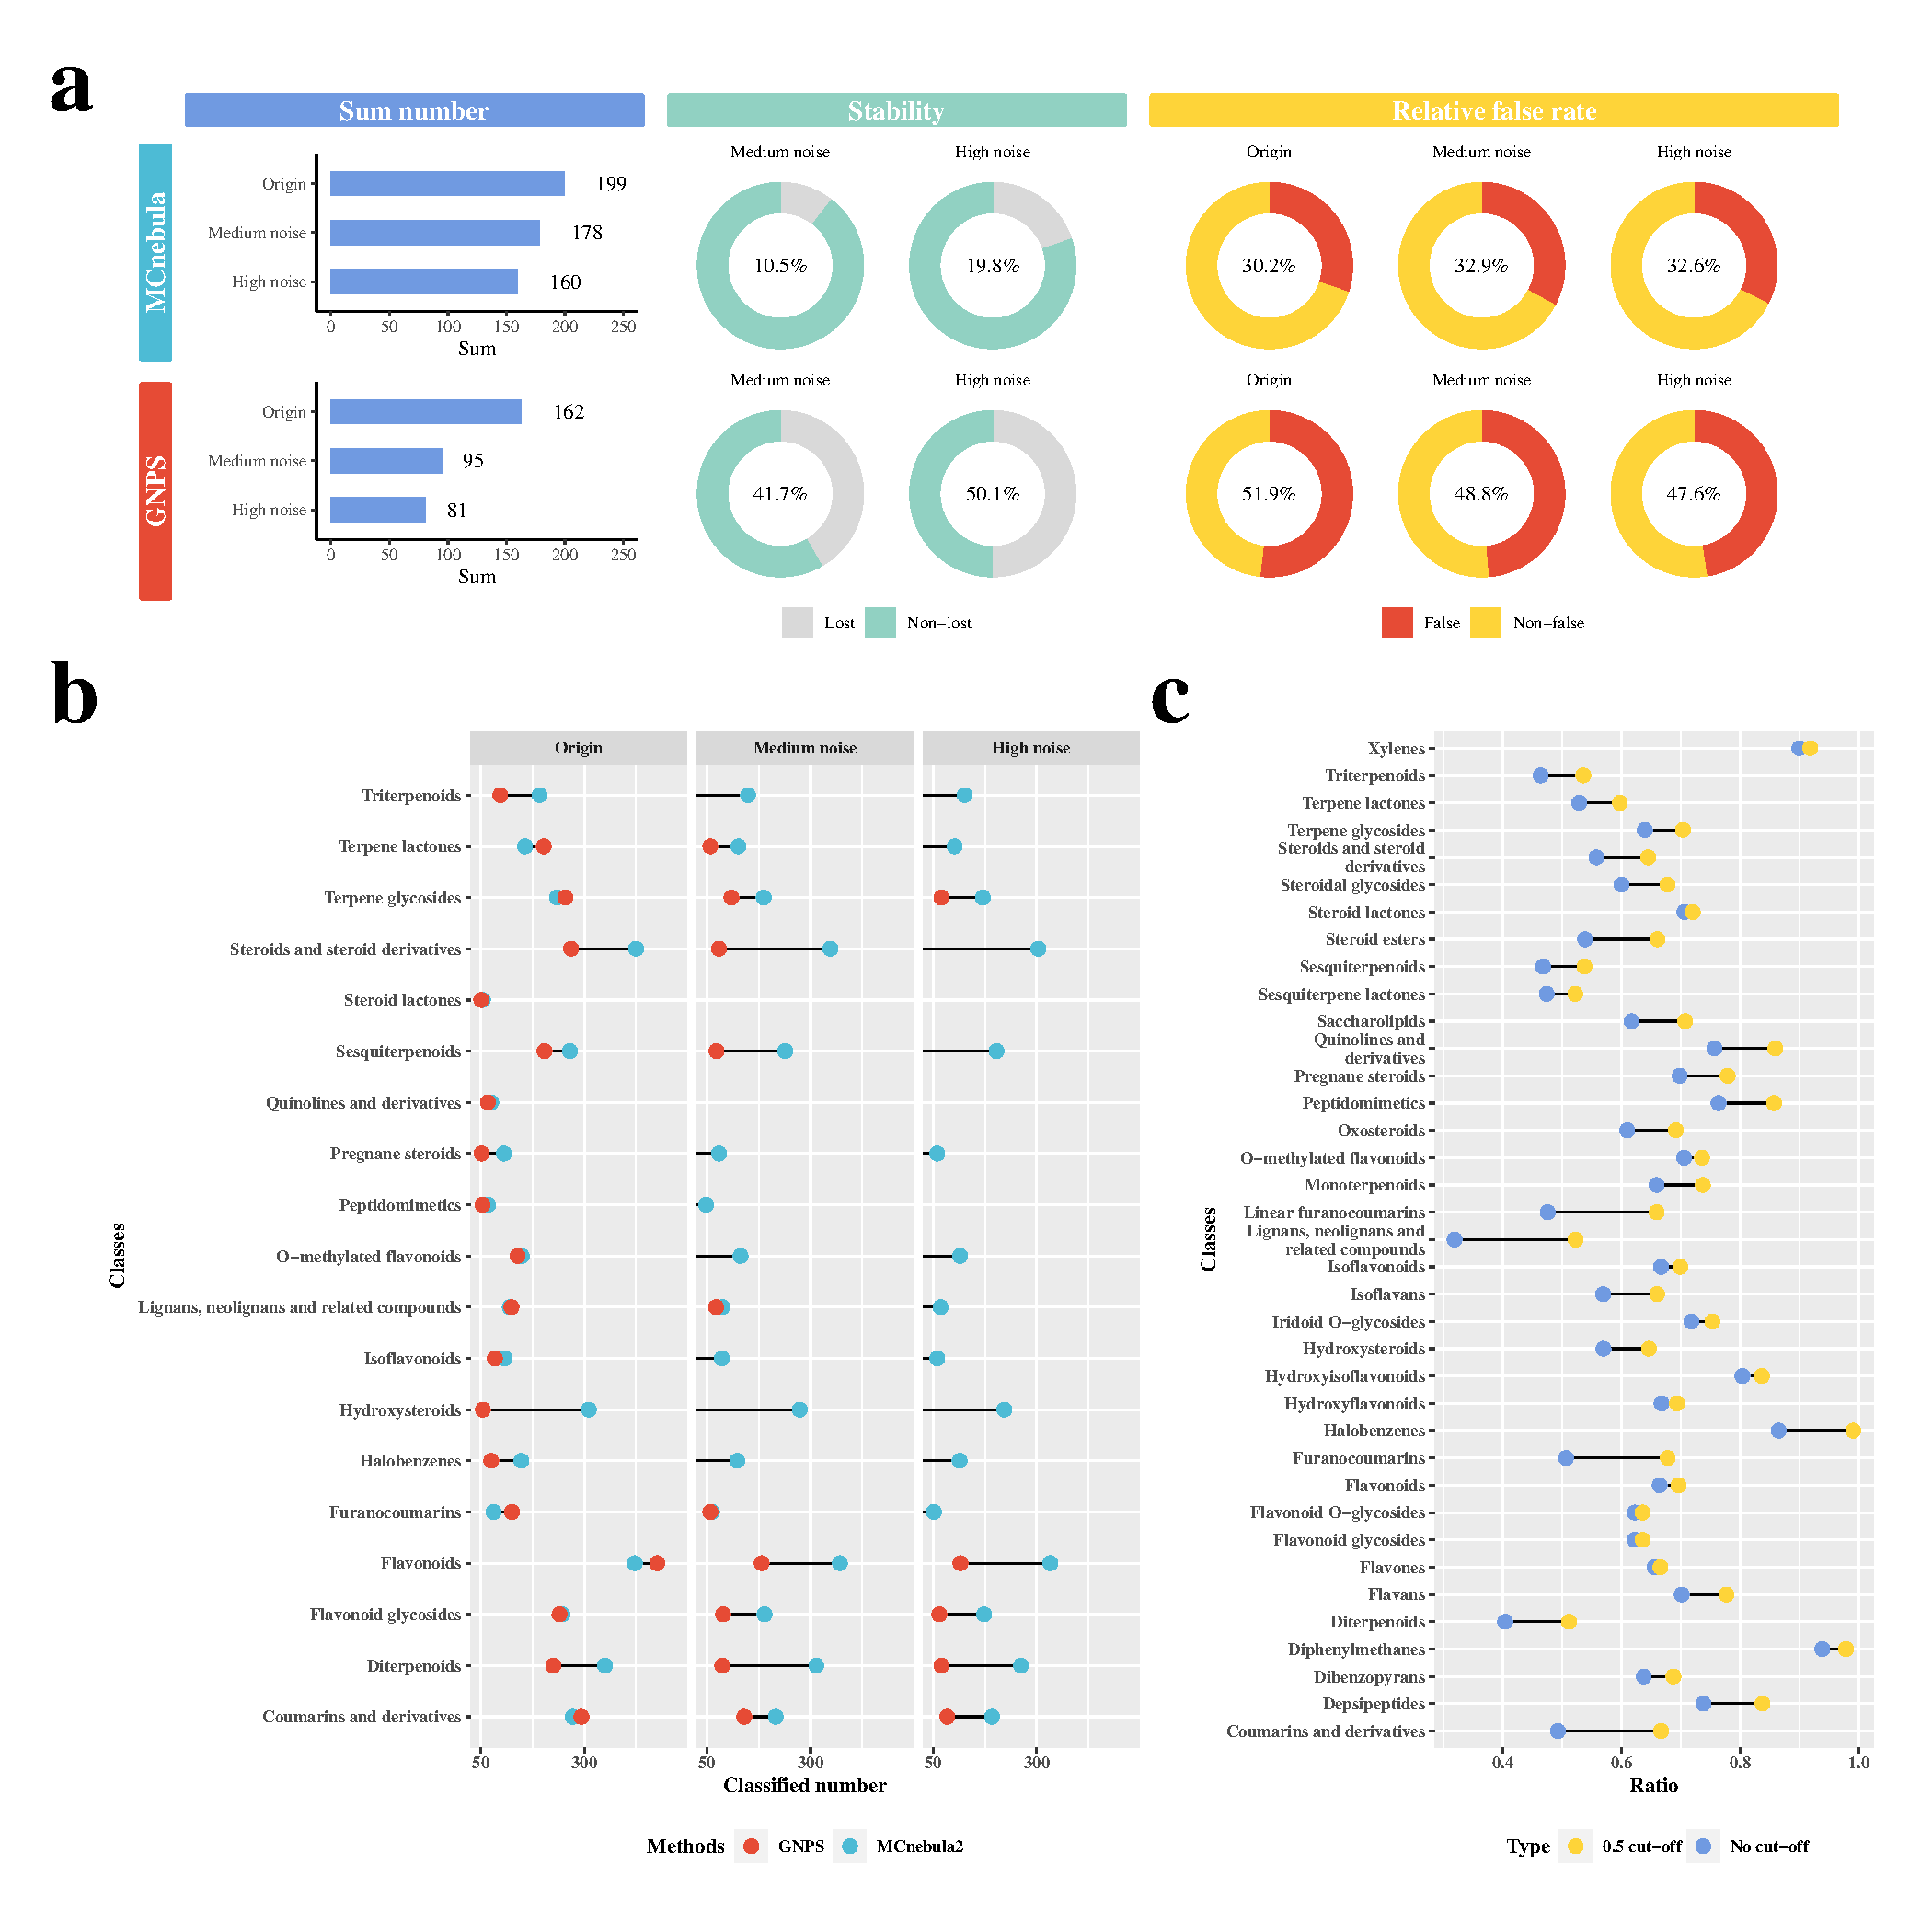
\includegraphics{fig3.compare_accuracy.pdf}
\caption{\textbf{Comparison of classifying of MCnebula with benchmark
method and Evaluation of identification accuracy of MCnebula}.
\textbf{a)} Fig.
{\protect\NoHyper\ref{fig:compare_accuracy}\protect\endNoHyper}a
illustrates the comparison of MCnebula and benchmark method (GNPS) with
three indicators: classified number, stability, relative false rate. The
classified number is calculated as average sum number of classified
compounds of the selected 19 chemical classes. The stability is
calculated as: \(S = (N_{origin} - N_{x}) / N_{origin}\) (\(N_{origin}\)
is the average sum number of origin dataset; \(N_{x}\) is the average
sum number of medium noise dataset or high noise dataset). The relative
false rate is calculated as: \(R = 1 - (1 - F) \times (1 - S)\) (\(F\)
is the absolute false rate; \(S\) is the stability, i.e., the average -
lost rate in stability assessment). \textbf{b)} Fig.
{\protect\NoHyper\ref{fig:compare_accuracy}\protect\endNoHyper}b
illustrates a comparison of classified number of MCnebula and benchmark
method. When noise is added into original dataset, some number of
classified features are occurred \textless{} 50, a cut-off (number
\(\geq\) 50) is set to exclude these classes from assessment.
\textbf{c)} Fig.
{\protect\NoHyper\ref{fig:compare_accuracy}\protect\endNoHyper}b
illustrates the identified accuracy of MCnebula. A cut-off (Tanimoto
similarity \(\geq\) 0.5) is set to get chemical structures of high
matching score for evaluation.}\label{fig:compare_accuracy}
}
\end{figure}

\textbf{Identified accuracy.} Using MCnebula workflow, the origin
dataset containing 8057 compounds (precursor ions m/z \textless{} 800),
all of these compounds were predicted with chemical molecular formulae,
and of these, 6610 compounds were predicted with chemical structure.
Those chemical structure were evaluated for accuracy in a classified
context. For the 37 chemical classes (Fig. \ref{fig:compare_accuracy}c),
the average false rate of identification was 37\%; the average
identified compounds number was 156. Among them, most of the identified
false rate were between 30\% to 40\%, however, some classes were quite
low, such as `Long-chain fatty acids' or `Lignans, neolignans and
related compounds'. The reliability of the predicted chemical structure
can be assessed in terms of a score. Tanimoto similarity provides such a
score for each predicted chemical structure (it provides the matching
degree of chemical fingerprints with structures). When Tanimoto
similarity sets the cutoff value to 0.5, the average false rate of
identification was 29.4\%; the average identified compounds number was
139 (Fig. \ref{fig:compare_accuracy}c). Above we evaluated the accuracy
of the identification of compounds in each chemical class obtained by
MCnebula. It should be noted that MCnebula itself does not contain any
module for identification, it only utilized the top scoring candidate
from the SIRIUS predicted results for annotation. For more evaluation on
identification please refer to the publication and our previous related
work\textsuperscript{\protect\hyperlink{ref-duhrkop_sirius_2019}{22},\protect\hyperlink{ref-lai_deep_2022}{50}}.

\hypertarget{data-analysis}{%
\paragraph{Data analysis}\label{data-analysis}}

\textbf{Serum metabolic analysis.} To illustrate the application of
MCnebula in metabolism, we re-analyzed the serum data from Wozniak et
al.\textsuperscript{\protect\hyperlink{ref-2020s}{42}}. The serum
samples were collected from patients in-hospital infected with
Staphylococcus aureus bacteremia (SaB) or not and healthy volunteers.
Overall, the samples were divided into 1) control groups, involving NN
(non-hospital, non-infected) and HN (hospital, non-infected); 2)
infection groups, involving HS (hospital, survival), HM (hospital,
mortality).

A total of 7680 `features' were detected while running with LC-MS
preprocessing on the serum dataset. After predicting the compounds by
MS/MS spectra (with SIRIUS software), subsequent analysis was performed
using MCnebula. Of these, 6501 `features' were annotated with predicted
molecular formula and further, 3449 `features' were annotated with
predicted chemical structure. Using ABC selection algorithm, we filtered
out more than one thousand chemical classes by applied of `inner filter'
module (see method section of ABC selection algorithm); further filtered
out 508 chemical classes while performing `cross filter'; for the
remaining 41 chemical classes, 19 chemical classes were manually
filtered out, while leaving the final 22 chemical classes to make up the
Nebula-Index, which further visualized as Child-Nebulae. It is worth
mentioning that the filtered out 527 (508 + 19) chemical classes could
be re-added to the analysis. Herein, with the basic workflow of
MCnebula, Parent-Nebula and Child-Nebulae were obtained (Fig. S1, Fig.
S2). By interrogating Child-Nebulae, we had a basic insight into the
chemical classes contained in the serum dataset. To mine more
information from Child-Nebulae: we performed a binary comparison of HS
and HM groups, ranking `features' according to Q-value (adjusted
P-value); the top 50 `features' were set as `tracers' to mark them in
Child-Nebulae (Fig. \ref{fig:serum_tracer}). By combining the features
selection algorithm about Q-value, the chemical classes exhibited in
Child-Nebulae were reduced. The log2(Fold Change) (log2(FC))
quantification for the HM versus HS groups was visualized in
Child-Nebulae (Fig. S3). In Fig. S3, the overall level of `Bile acids,
alcohols and derivatives' (BAs) class and `Acyl carnitines' (ACs) (Fig.
\ref{fig:ac_node2}a and b) class increased remarkably, while the overall
level of `Lysophosphatidylcholines' (LPCs) class decreased remarkably.
Indeed, BAs, ACs and LPCs were reported associated with liver
dysfunction, imbalance of intestinal microphylactic homeostasis, and
mortality
risk\textsuperscript{\protect\hyperlink{ref-2020s}{42},\protect\hyperlink{ref-2021db}{51},\protect\hyperlink{ref-2016at}{52}}.

\begin{figure}
\hypertarget{fig:serum_tracer}{%
\centering
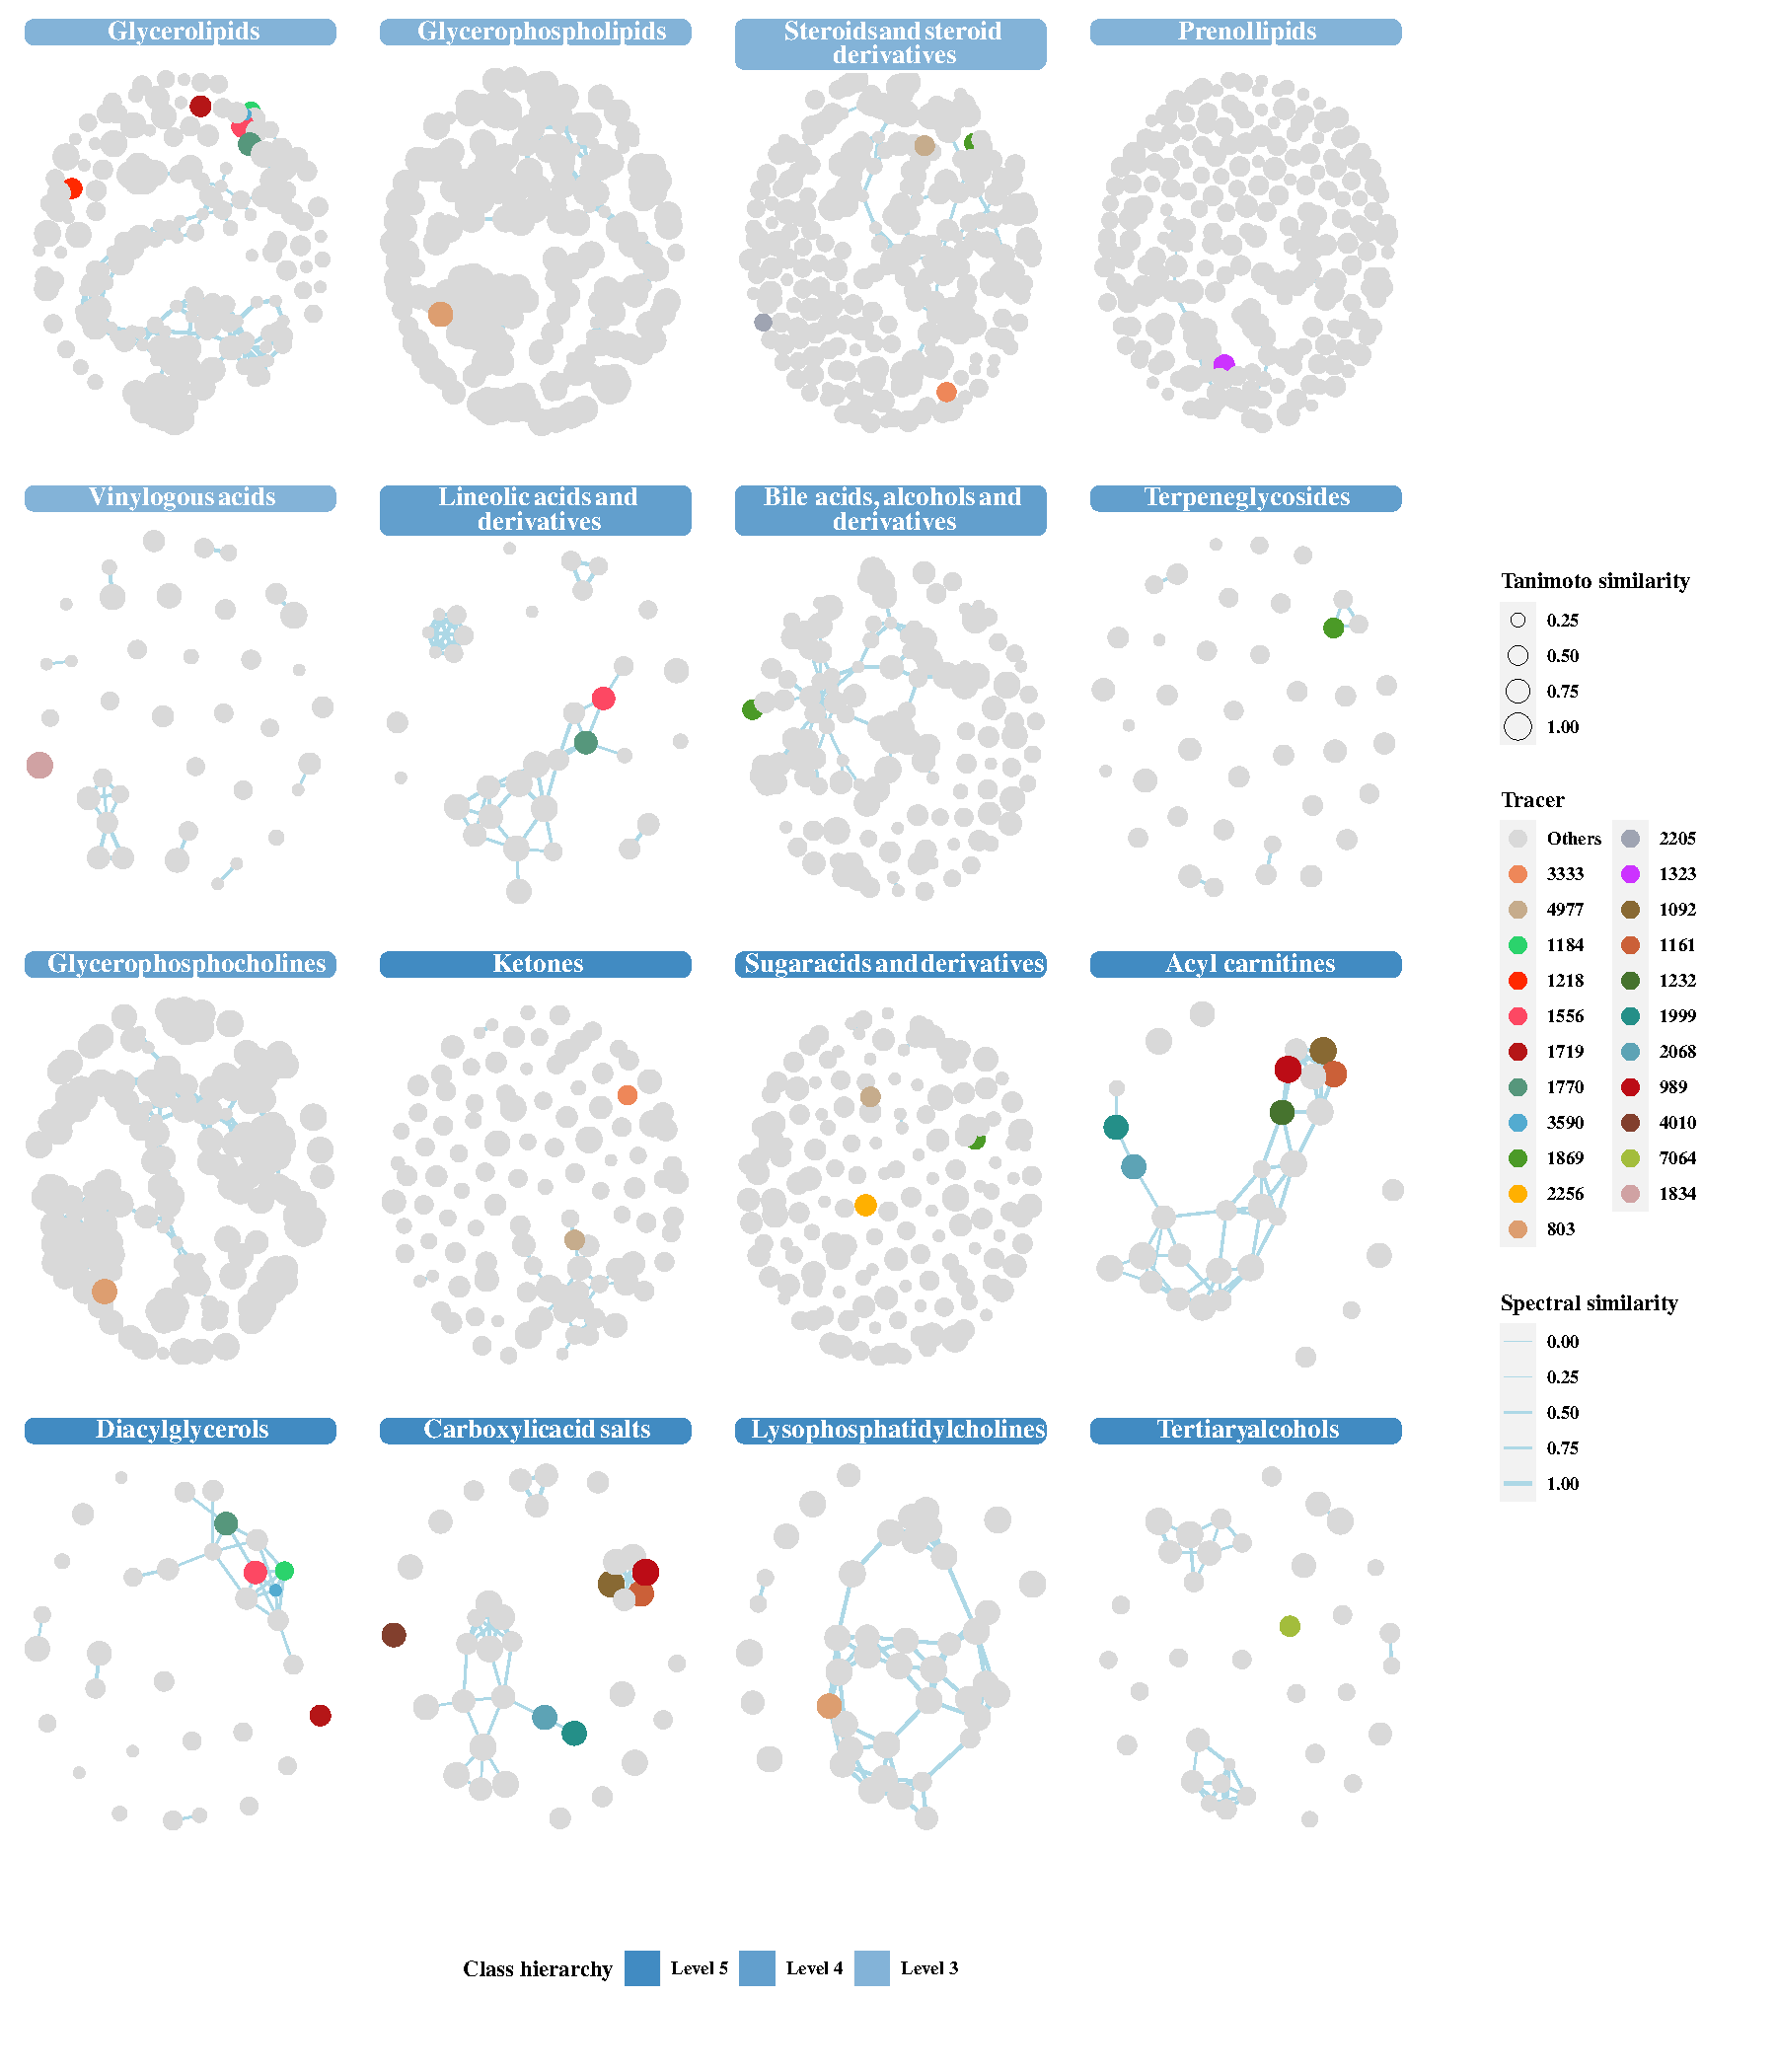
\includegraphics{fig4.serum_tracer.pdf}
\caption{\textbf{Tracing top `features' in Child-Nebulae of serum
metabolomics dataset.} According to the rankings of `features' by
statistic analysis, the top `features' are marked with different colors
in Child-Nebulae.}\label{fig:serum_tracer}
}
\end{figure}

\begin{figure}
\hypertarget{fig:ac_node2}{%
\centering
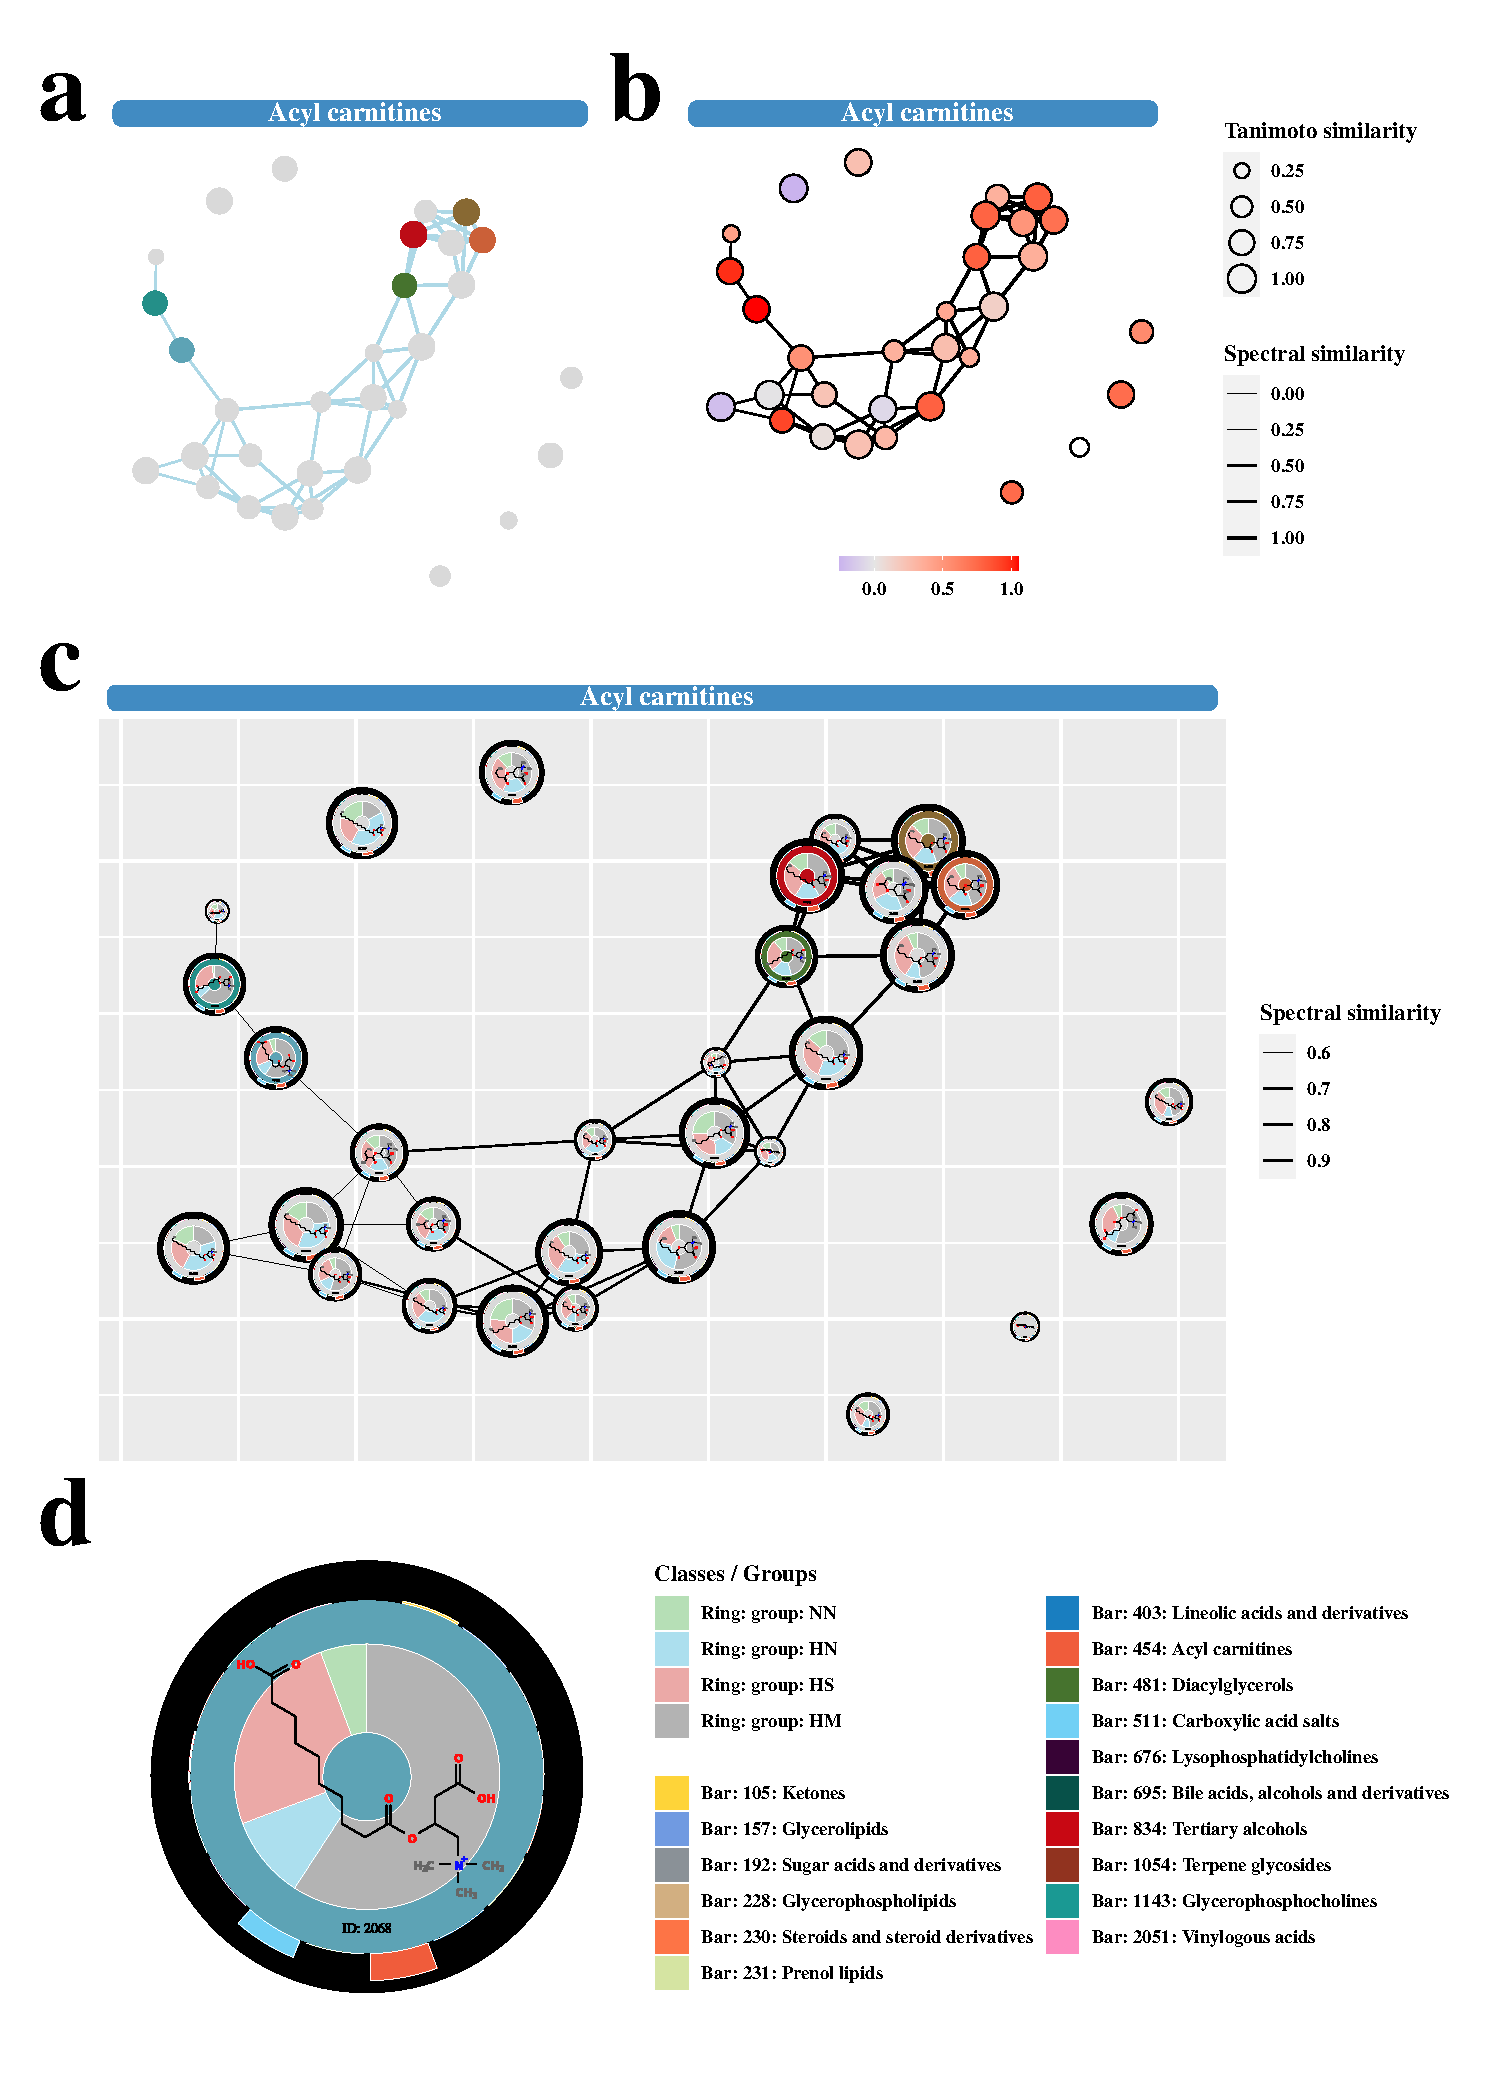
\includegraphics{fig5.ac_node2.pdf}
\caption{\textbf{In-depth visualization of Child-Nebula of `Acyl
carnitines'} \textbf{a)}, refer to Fig.
{\protect\NoHyper\ref{fig:serum_tracer}\protect\endNoHyper}. \textbf{b)}
The log\textsubscript{2}(Fold change) value of HM versus HS group is
shown in Child-Nebulae as gradient color. The nodes with white color
indicate `features' with missing quantification value (these `features'
were detected in our re-analysis, but not in Wozniak et al.).
\textbf{c)} The nodes of top `features' are marked with color. The nodes
of `features' are annotated with structures, ring diagram and bar plot
of posterior probability of classes prediction (PPCP). The top candidate
of Chemical structure of `features' are mapped into nodes. The Ring
diagram map relative summed peak area of per `feature' detected within
each metadata group (NN: non-hospital, non-infected; HN: hospital,
non-infected; HS: hospital, survival; HM: hospital, mortality). The
nodes without ring diagram indicate `features' with missing
quantification value (these `features' were detected in our re-analysis,
but not in Wozniak et al.) The Bar plot map PPCP of structural
(sub-structural or dominant structural) classes for the `feature'.
\textbf{d)} The zoom in node of `feature' 2068 (ID) and its
legend.}\label{fig:ac_node2}
}
\end{figure}

By deep annotation of Child-Nebula, all three classes of compounds have
similar structural parent nuclei, and their levels in the NN, HN, HS,
and HM groups are similar (Fig. \ref{fig:ac_node2}c, Fig. S4).
Subsequently, we performed cluster heat map analysis and pathway
enrichment analysis on the compounds of these three classes. As shown in
the clustering heat map (Fig. \ref{fig:hps}), the control group of ACs
and BAs were remarkably separated from the infection group, which
implied the infection relevance of ACs and BAs to SaB. In contrast, LPCs
did not show remarkable SaB infection relevance or mortality relevance,
probably owing to the general consistency of this class of compounds for
SaB disease. We performed pathway enrichment analysis for these three
classes of significant compounds (HS versus HM group, Q-value
\textless{} 0.05). The results of BAs showed that four compounds
exhibited metabolic pathways associated with `Bile secretion',
`Cholesterol metabolism', and `Primary bile acid biosynthesis' etc (Fig.
S5b). Among them, \(beta\)GCS was a class of compounds with the same
parent nucleus. The results for LPCs suggested that compounds with
similar parent nucleus structure of LPCs implied association with a
series of downstream pathways (Fig. S5c). The significant compounds of
ACs were not enriched in the pathway. But, A fundamental role of ACs in
tuning the switch between the glucose and fatty acid metabolism was
reviewed\textsuperscript{\protect\hyperlink{ref-2018bi}{53}}. Their
function implemented via bi-directional transport of acyl moieties
Between cytosol and mitochondria (Fig. S5a).

\begin{figure}
\hypertarget{fig:hps}{%
\centering
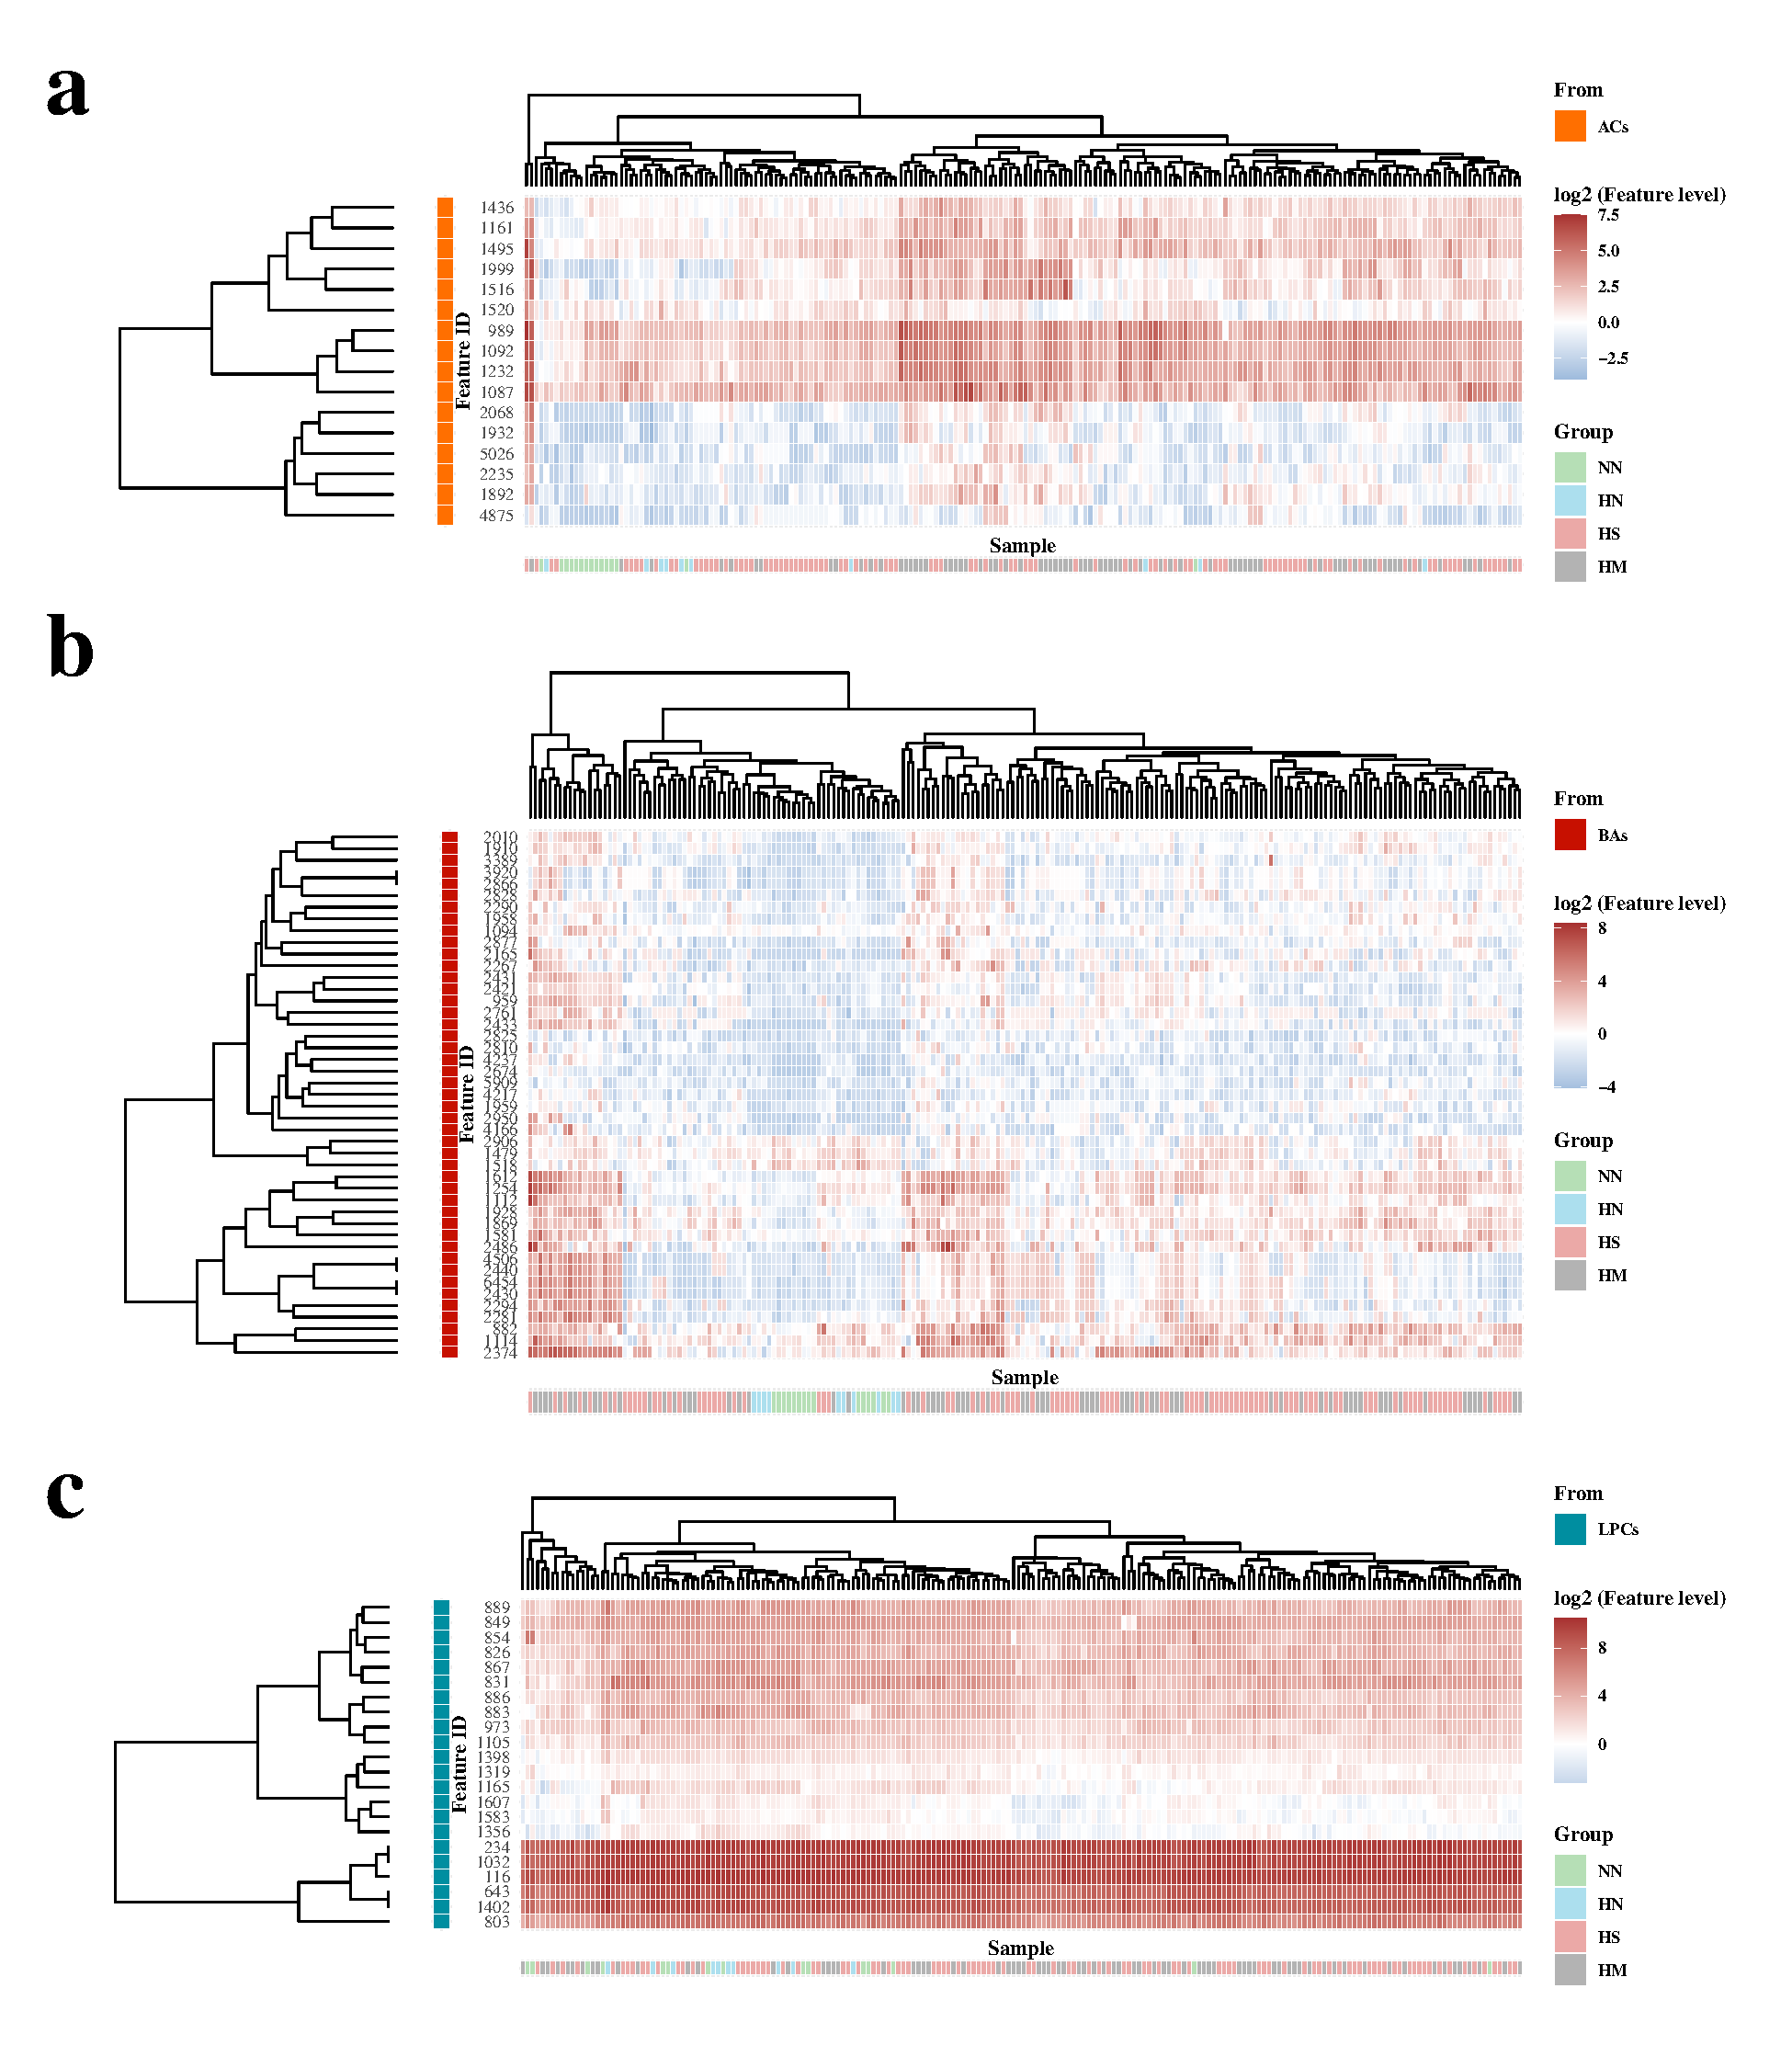
\includegraphics{fig6.hps.pdf}
\caption{\textbf{Heat maps of `Acyl carnitines' (ACs),
`Lysophosphatidylcholines' (LPCs), `Bile acids, alcohols and
derivatives' (BAs) in serum metabolomics dataset.} Figure
{\protect\NoHyper\ref{fig:hps}\protect\endNoHyper}\textbf{a}, \textbf{c}
and \textbf{e} show heat maps of level of ACs, LPCs and BAs. The
`features' are select by either in infection groups versus control
groups or HM versus HS group: Q-value \textless{} 0.05,
\textbar log\textsubscript{2}(FC)\textbar{} \(\geq\)
0.3.}\label{fig:hps}
}
\end{figure}

In research of Wozniak et
al\textsuperscript{\protect\hyperlink{ref-2020s}{42}}, five ACs
compounds were identified. In addition, four top metabolites
(2-Hexadecanoylthio-1-Ethylphosphorylcholine (HEPC);
sphingosine-1-phosphate (S1P); decanoyl-carnitine; L-Thyroxine (T4))
were also identified. In our reanalysis, all identifications were in
line except for HEPC (see `Data and code availability' section for the
report of serum dataset analysis). In our re-analysis, `HEPC' was
identified as 1-pentadecanoyl-sn-glycero-3-phosphocholine (LPC15:0) or
its stereoisomers. Indeed, HEPC and LPC15:0 are quite similar in
structure, but distinct in element constitution (corresponding to
C\textsubscript{23}H\textsubscript{48}NO\textsubscript{5}PS and
C\textsubscript{23}H\textsubscript{48}NO\textsubscript{7}P
respectively). They were clearly distinct in terms of chemical
classification. HEPC belongs to `Cholines' (level 5) from `Organic
nitrogen compounds' (superclass) family, whereas LPC15:0 belongs to
`Lysophosphatidylcholines' (level 5) from `Lipids and lipid-like
molecules' family. As a part of MCnebula workflow, sulfur element is
detectable for SIRIUS in isotopes pattern with high mass
accuracy\textsuperscript{\protect\hyperlink{ref-bocker_sirius_2009}{37}}.
However, for the MS/MS spectra of `HEPC', there was no candidate formula
that containing sulfur element. Overall, we identified more compounds
with the MCnebula workflow and many of the results were in line with the
analysis of Wozniak et
al\textsuperscript{\protect\hyperlink{ref-2020s}{42}}. All identified
compounds were collated in Tab. S2 (filtered with Tanimoto similarity
\textgreater{} 0.5 and de-duplicated with the first hash block of
InChIKey (molecular skeleton)). The compounds (top 50 of EFS and MWU)
that were not successfully identified via spectral library matching by
Wozniak et al.~but were identified by our MCnebula workflow for
molecular formula or chemical structure were additionally collated (Tab.
S3).

\textbf{Herbal medicine analysis.} We used MCnebula to interpretate
structure diversity and chemical transformation during traditional
processing of a representative herbal medicine, \emph{Eucommiae Cortex,}
the peel of \emph{Eucommia ulmoides Oliv. (E.
ulmoides)}\textsuperscript{\protect\hyperlink{ref-2021n}{54}}. After
being processed with saline water, it is commonly applied to treat renal
diseases for a long time in China but the chemical basis still remained
to be explored. With the help of ABC selection algorithm in MCnebula, a
total of 29 chemical classes representing the richness of composition of
E. ulmoides were obtained. Two groups of quantification data were
performed with binary comparison. The top 20 features (Top20) were
selected using function `select\_features' (\textbar Log2(Fold
change)\textbar{} \textgreater{} 0.3, Q-value \textless{} 0.05, Tanimoto
similarity \textgreater{} 0.5) and were traced in Child-Nebulae (Fig.
S6). We used MCnebula to draw the mirrored match of MS/MS spectra and
extracted ions chromatography (EIC) plots of the Top20 (Fig. S7 and S8).
According to Fig. S8, we speculated that the `features' of ID 1642,
1785, and 2321 were newly generated compounds because the peak area
levels before the processing were almost zero compared to those after
processing. Their chemical structures are showed in Fig. S7. Among them,
the `feature' of ID 1642 has a higher probability of correct
identification (Tanimoto similarity: 0.69). Based on Fig. S6, we knew
that `feature' of ID 1642 belongs to `Iridoids and derivatives' (IAD),
the others were `Dialkyl ethers' (DE; ID 1785) and `Phenylpropanoids and
polyketides' (PAP; ID 2321). We annotated in depth of the Child-Nebulae
of IAD, DE and PAP respectively. The locations of the `features' of ID
1642, 1785 and 2321 in the Child-Nebulae were interrogated (Fig. S9a, b,
and c). Only the `features' of ID 1642 had neighboring `features' and
their identified chemical structures (ID 2110 and ID 854) had similar
parent nuclei. The `features' of ID 2110 and ID 854 were identified with
chemical structure (Tanimoto similarity: 0.69 and 0.7 respectively)
(Fig. S9d, e, and f); their levels of peak area were decreased and
increased after the processing. Based on the chemical structures shown
in Fig. S9d and e, we speculated that the compound of ID 2110 was
partially converted to the compound of ID 854 after the processing,
which may involve chemical changes such as dehydration and
rearrangement. Such speculation explained the alteration of the levels
of peak area. In addition, the increasement in the level of the compound
ID 1642 (its spectra were shown in Fig. S7 and S8) may also be
associated with the reduction of the compound ID 2110.

The methods of MCnebula we have demonstrated for discovering significant
compounds and discovering chemical changes can be applied to explore
more compounds in Tab. S4, but we would not expand on this description
here.

\hypertarget{discussion}{%
\subsubsection{Discussion}\label{discussion}}

The analysis of LC-MS/MS data is challenging because of its large
dataset and the potential information of the unknown compounds as well
as the limited of reference spectral library. Researchers often need to
take much time on mapping the landscape of all the interesting compounds
from this ``black box'', and then move to next step in research MCnebula
could assist researchers in focusing on potential markers or interesting
compounds quickly by combining full-spectrum identification with machine
prediction, visualization of sub-nebulae in a multi-dimensional view,
and statistical analysis to track top `features' and find analogues. The
ABC selection algorithm can summarize a representative chemical class in
a dataset and obtain the features to that class, so the overall
direction of the study is unbiased. Also, it is an effective guarantee
for statistical analysis to produce top features for tracing analysis in
next step. The results of statistical analysis based on feature level
may cause bias since the loss of information, filtering on the basis of
chemical classes level can prevent the bias in some degree. The
Child-Nebula, which mapped on the basis of the chemical classes obtained
by the ABC selection algorithm, achieved the goal of visualizing the
huge untargeted dataset as a single graph. Above all, the parameters of
the ABC selection algorithm were subjectively adjustable and they should
be determined according to the richness of the chemical class of the
studied object. In general, our default parameters used to acquire the
chemical classes that are abundant in variety according to the datasets
and filtered out those that were too large or too small classes in
conceptual scope.

For identification, spectral library matching is still the main method
for LC-MS/MS data because of its high accuracy. The general classifying
of compounds is also based on it, i.e., the chemical structure is
firstly identified by spectral matching, and then its chemical class is
evaluated based on the chemical structure. Considering the limit of
reference spectral library, The classifying technique like
CANOPUS\textsuperscript{\protect\hyperlink{ref-duhrkop_systematic_2021}{34}}incorporated
in MCnebula bypassed the first step of identifying the chemical
structure but predicted the possible chemical class even if the exact
chemical structure was not known. MCnebula combined this cutting-edge
technology with ABC selection algorithm and achieve visualization of
Child-Nebulae, which make it possible to explore unknown compounds that
beyond spectral library. We compared the classifying method of MCnebula
with GNPS, of which method relies on chemical structure identification.
When different levels of noise were added, the number of classified
compounds of GNPS decreased remarkably compared with the stable
performance of MCnebula. For the actual acquired MS/MS spectra, they
were not as good as the reference spectra and contained some noise.
Indeed ,the reality of MS/MS spectra is much closer to the condition
with noise. It means MCnebula can resist noise interference in some
extent. At the end of the evaluation, we examined the accuracy of the
identification by MCnebula. It confirmed that the accuracy of
identification fluctuated around 70\%, which was the same as
SIRIUS\textsuperscript{\protect\hyperlink{ref-duhrkop_sirius_2019}{22}}.

Serum metabolomics data was applied to illustrate that MCnebula can be
used for pathway analysis and biomarker discovery. Most of our results
were consistent with that of
reference\textsuperscript{\protect\hyperlink{ref-2020s}{42}}. The
exciting thing was that that we identified more metabolites that beyond
the scope of spectral library matching. Three of the four top
metabolites identified by Wozniak et al.~were the same as our
re-identification, but only one metabolite was controversial. Wozniak et
al.~mentioned ACs compounds had correlation with SaB disease and ACs
compounds were also re-identified in our study. Wozniak et al.~used a
joint approach of Ensemble Feature Selection (EFS) and Mann-Whitney U
(MWU) tests to screen top
metabolites\textsuperscript{\protect\hyperlink{ref-2020s}{42}}. When we
compared the 50 top `features' obtained by the `binary comparison'
method integrated in MCnebula with the top 50 metabolites (top 50 of EFS
and 50 of MWU) obtained by the joint method of W et al., a total of 37
overlapped metabolites were screened out, including the key metabolite
of L-Thyroxine in the reference study.~Top `features' were usually
different according to the feature selection algorithm. The reliability
of the `binary comparison' method was verified again by our ranked
results comparing with those of Wozniak et al.~In addition to the
consistent parts, , more interesting results about other chemical
classes associated with SaB disease were revealed by MCnebula. We
discovered additional classes, i.e.~`Lysophosphatidylcholines' (LPCs)
and `Bile acids, alcohols and derivatives' (BAs), that were not
concerned in previous study. Acutally, LPCs have been extensively
investigated in the context of inflammation and atherosclerosis
development\textsuperscript{\protect\hyperlink{ref-2016at}{52},\protect\hyperlink{ref-2020cv}{55},\protect\hyperlink{ref-2014ao}{56}}.
In a recent review\textsuperscript{\protect\hyperlink{ref-2020cv}{55}},
the complex roles of LPCs in vascular inflammation were well described,
involving the context-dependent pro- or anti-inflammatory action, impact
in innate immune cells and adaptive immune system, etc. Decreasing level
of LPCs was associated with wild range of diseases of increasing
mortality risk\textsuperscript{\protect\hyperlink{ref-2016at}{52}}. The
investigation of spesis indicated LPCs concentrations in blood were
established correlation with severe sepsis or septic
shock\textsuperscript{\protect\hyperlink{ref-2014ao}{56}}. LPCs was
reported inversely correlated with mortality in sepsis
patients\textsuperscript{\protect\hyperlink{ref-2003n}{57}}. BAs'
disorder implied a liver dysfunction and imbalance of intestinal
microphylactic
homeostasis\textsuperscript{\protect\hyperlink{ref-2021dg}{58}}. The
chemical multiversity of BAs, which were discovered in the BAs'
child-nebula, were determined by the intestinal microbiome and allowed
for a complex regulation of adaptive responses in host. In our study,
the level of BAs showed higher correlation with SaB infection than ACs.
The decreased level of LPCs suggested a mortality risk of SaB infection.
From LPCs to BAs, steroids related classes, `Lineolic acids and
derivatives', and other fatty acids related classes, showed that liver
played a central role in SaB infection and mortality. Liver X receptors
(LXRs) played pivotal roles in the transcriptional control of lipid
metabolism\textsuperscript{\protect\hyperlink{ref-2018bd}{59}}. LXRs
modulated membrane phospholipid composition through activation of
lysophosphatidylcholine acyltransferase 3 (LPCAT3), which was directly
related to LPCs\textsuperscript{\protect\hyperlink{ref-2021di}{60}}. The
above classes showed correlation with
LXRs\textsuperscript{\protect\hyperlink{ref-2018bd}{59}}. Unfortunately,
LXRs' specific role in SaB infection or mortality has not been reported
and beyond the scope of this research.

In herbal dataset analysis, MCnebula provided a quick annotation of
compounds and exploration of chemical changes in Child-Nebulae with a
scope of chemical classes. The main components of \emph{E. ulmoides}
were lignans, iridoids, phenolics, flavonoids, steroid and
terpenoids\textsuperscript{\protect\hyperlink{ref-huang_traditional_2021}{61}}.
In our study, the chemical classes that obtained by ABC selection
algorithm included `Lignans, neolignans and related compounds' (LNARC)
and `Iridoids and derivatives' (IAD), as well as `Monoterpenoids' and
`Terpene glycosides'. The flavonoids were covered by `Phenylpropanoids
and polyketides' (PAP)\textsuperscript{\protect\hyperlink{ref-2016}{24}}
and phenolics may be found in `Methoxyphenols'. The flavonoids were
similar to the steroids and were not retained in selected results as
`Flavonoides' and `Steroids and steroid derivatives', because they were
not as abundant in \emph{E. ulmoides} (bark) as LNARC and IAD. Many of
the compounds that identified in chemical classes of LNARC and IAD (Tab.
S1) were reported in previous research about LC-MS/MS analysis of
\emph{E.
ulmoides}\textsuperscript{\protect\hyperlink{ref-2014w}{62},\protect\hyperlink{ref-2015v}{63}}.
We obtained top features based on statistical comparison of the changes
in `features' quantification levels before and after processing. One of
the compounds that changed significantly or even was newly produced (ID:
1642) was traced in the Child-Nebulae. We hypothesized that it was
related to two structurally similar compounds by transformation. The
application of MCnebula in the analysis of plant-derived compounds was
well illustrated with this example, particular for quick identification
and exploration of chemical changes. Notably, the reference spectral
library or database for plant-derived compounds was much more scarce
compared with reference spectral library for human-derived metabolites,
Although some specific database of plant-derived compounds was
constructed\textsuperscript{\protect\hyperlink{ref-2012ac}{64}}, there
were lack of enough fragmentation spectra for comprehensive library
match. With the help of MCnebula, a rapid and reliable resolution of
complex compositions of plant-derived can be achieved.

\hypertarget{conclusion}{%
\subsection{Conclusion}\label{conclusion}}

The analysis of LC-MS/MS data is challenging because of its large
dataset and much information of the unknown compounds as well as the
limited of reference spectral library. Thus, we established a framework
called MCnebula to facilitate mass spectrometry data analysis by
focusing on critical chemical classes and visualization in multiple
dimensions. MCnebula was proposed and implemented in the R language with
package of MCnebula. As an integrated visualization method, MCnebula may
be more popular for researchers without background of bioinformatics and
computer science. According to the results of method evaluation,
MCnebula had a lower relative false rate of classified accuracy and its
accuracy of identification was up to 70\%. In order to illustrate the
broad utility of MCnebula, we investigated a human-derived serum dataset
for metabolomics analysis. The results indicated that `Acyl carnitines'
were screened out by tracing structural classes of biomarkers which was
consistent with the reference. We also investigated a plant-derived
dataset of herbal E. ulmoides to achieve a rapid unknown compound
annotation and discovery. MCnebula has a great potential in the field of
chemistry and biology. In the future, we hope that fields of application
of MCnebula could expand to agriculture, food science, medicine and so
on.

\hypertarget{acknowledgements}{%
\subsection{Acknowledgements}\label{acknowledgements}}

This work was financially supported by the National Natural Science
Foundation of China (No.~81922073), Zhejiang Province Traditional
Chinese Medicine Science and Technology Project (Nos. 2022ZQ033).

\hypertarget{bibliography}{%
\section*{Reference}\label{bibliography}}
\addcontentsline{toc}{section}{Reference}

\hypertarget{refs}{}
\begin{CSLReferences}{0}{0}
\leavevmode\vadjust pre{\hypertarget{ref-2020p}{}}%
\CSLLeftMargin{(1) }%
\CSLRightInline{Tsugawa, H.; Ikeda, K.; Takahashi, M.; Satoh, A.; Mori,
Y.; Uchino, H.; Okahashi, N.; Yamada, Y.; Tada, I.; Bonini, P.; Higashi,
Y.; Okazaki, Y.; Zhou, Z.; Zhu, Z.-J.; Koelmel, J.; Cajka, T.; Fiehn,
O.; Saito, K.; Arita, M.; Arita, M. A Lipidome Atlas in {MS-DIAL} 4.
\emph{Nature Biotechnology} \textbf{2020}, \emph{38} (10), 1159--1163.
\url{https://doi.org/10.1038/s41587-020-0531-2}.}

\leavevmode\vadjust pre{\hypertarget{ref-2018az}{}}%
\CSLLeftMargin{(2) }%
\CSLRightInline{Chong, J.; Soufan, O.; Li, C.; Caraus, I.; Li, S.;
Bourque, G.; Wishart, D. S.; Xia, J. {MetaboAnalyst} 4.0: Towards More
Transparent and Integrative Metabolomics Analysis. \emph{Nucleic Acids
Research} \textbf{2018}, \emph{46} (W1), W486--W494.
\url{https://doi.org/10.1093/nar/gky310}.}

\leavevmode\vadjust pre{\hypertarget{ref-2020co}{}}%
\CSLLeftMargin{(3) }%
\CSLRightInline{Tsugawa, H. Computational {MS}/{MS Fragmentation} and
{Structure Elucidation Using MS-FINDER Software}. In \emph{Comprehensive
{Natural Products III}}; {Elsevier}, 2020; pp 189--210.
\url{https://doi.org/10.1016/B978-0-12-409547-2.14645-1}.}

\leavevmode\vadjust pre{\hypertarget{ref-2016a}{}}%
\CSLLeftMargin{(4) }%
\CSLRightInline{Wang, M.; Carver, J. J.; Phelan, V. V.; Sanchez, L. M.;
Garg, N.; Peng, Y.; Nguyen, D. D.; Watrous, J.; Kapono, C. A.;
Luzzatto-Knaan, T.; Porto, C.; Bouslimani, A.; Melnik, A. V.; Meehan, M.
J.; Liu, W.-T.; Crüsemann, M.; Boudreau, P. D.; Esquenazi, E.;
Sandoval-Calderón, M.; Kersten, R. D.; Pace, L. A.; Quinn, R. A.;
Duncan, K. R.; Hsu, C.-C.; Floros, D. J.; Gavilan, R. G.; Kleigrewe, K.;
Northen, T.; Dutton, R. J.; Parrot, D.; Carlson, E. E.; Aigle, B.;
Michelsen, C. F.; Jelsbak, L.; Sohlenkamp, C.; Pevzner, P.; Edlund, A.;
McLean, J.; Piel, J.; Murphy, B. T.; Gerwick, L.; Liaw, C.-C.; Yang,
Y.-L.; Humpf, H.-U.; Maansson, M.; Keyzers, R. A.; Sims, A. C.; Johnson,
A. R.; Sidebottom, A. M.; Sedio, B. E.; Klitgaard, A.; Larson, C. B.;
Boya P, C. A.; Torres-Mendoza, D.; Gonzalez, D. J.; Silva, D. B.;
Marques, L. M.; Demarque, D. P.; Pociute, E.; O'Neill, E. C.; Briand,
E.; Helfrich, E. J. N.; Granatosky, E. A.; Glukhov, E.; Ryffel, F.;
Houson, H.; Mohimani, H.; Kharbush, J. J.; Zeng, Y.; Vorholt, J. A.;
Kurita, K. L.; Charusanti, P.; McPhail, K. L.; Nielsen, K. F.; Vuong,
L.; Elfeki, M.; Traxler, M. F.; Engene, N.; Koyama, N.; Vining, O. B.;
Baric, R.; Silva, R. R.; Mascuch, S. J.; Tomasi, S.; Jenkins, S.;
Macherla, V.; Hoffman, T.; Agarwal, V.; Williams, P. G.; Dai, J.;
Neupane, R.; Gurr, J.; Rodríguez, A. M. C.; Lamsa, A.; Zhang, C.;
Dorrestein, K.; Duggan, B. M.; Almaliti, J.; Allard, P.-M.; Phapale, P.;
Nothias, L.-F.; Alexandrov, T.; Litaudon, M.; Wolfender, J.-L.; Kyle, J.
E.; Metz, T. O.; Peryea, T.; Nguyen, D.-T.; VanLeer, D.; Shinn, P.;
Jadhav, A.; Müller, R.; Waters, K. M.; Shi, W.; Liu, X.; Zhang, L.;
Knight, R.; Jensen, P. R.; Palsson, B. Ø.; Pogliano, K.; Linington, R.
G.; Gutiérrez, M.; Lopes, N. P.; Gerwick, W. H.; Moore, B. S.;
Dorrestein, P. C.; Bandeira, N. Sharing and Community Curation of Mass
Spectrometry Data with {Global Natural Products Social Molecular
Networking}. \emph{Nature Biotechnology} \textbf{2016}, \emph{34} (8),
828--837. \url{https://doi.org/10.1038/nbt.3597}.}

\leavevmode\vadjust pre{\hypertarget{ref-2012d}{}}%
\CSLLeftMargin{(5) }%
\CSLRightInline{Chambers, M. C.; Maclean, B.; Burke, R.; Amodei, D.;
Ruderman, D. L.; Neumann, S.; Gatto, L.; Fischer, B.; Pratt, B.;
Egertson, J.; Hoff, K.; Kessner, D.; Tasman, N.; Shulman, N.; Frewen,
B.; Baker, T. A.; Brusniak, M.-Y.; Paulse, C.; Creasy, D.; Flashner, L.;
Kani, K.; Moulding, C.; Seymour, S. L.; Nuwaysir, L. M.; Lefebvre, B.;
Kuhlmann, F.; Roark, J.; Rainer, P.; Detlev, S.; Hemenway, T.; Huhmer,
A.; Langridge, J.; Connolly, B.; Chadick, T.; Holly, K.; Eckels, J.;
Deutsch, E. W.; Moritz, R. L.; Katz, J. E.; Agus, D. B.; MacCoss, M.;
Tabb, D. L.; Mallick, P. A Cross-Platform Toolkit for Mass Spectrometry
and Proteomics. \emph{Nature Biotechnology} \textbf{2012}, \emph{30}
(10), 918--920. \url{https://doi.org/ghh626}.}

\leavevmode\vadjust pre{\hypertarget{ref-2016e}{}}%
\CSLLeftMargin{(6) }%
\CSLRightInline{Röst, H. L.; Sachsenberg, T.; Aiche, S.; Bielow, C.;
Weisser, H.; Aicheler, F.; Andreotti, S.; Ehrlich, H.-C.; Gutenbrunner,
P.; Kenar, E.; Liang, X.; Nahnsen, S.; Nilse, L.; Pfeuffer, J.;
Rosenberger, G.; Rurik, M.; Schmitt, U.; Veit, J.; Walzer, M.; Wojnar,
D.; Wolski, W. E.; Schilling, O.; Choudhary, J. S.; Malmström, L.;
Aebersold, R.; Reinert, K.; Kohlbacher, O. {OpenMS}: A Flexible
Open-Source Software Platform for Mass Spectrometry Data Analysis.
\emph{Nature Methods} \textbf{2016}, \emph{13} (9), 741--748.
\url{https://doi.org/f82r32}.}

\leavevmode\vadjust pre{\hypertarget{ref-2006a}{}}%
\CSLLeftMargin{(7) }%
\CSLRightInline{Smith, C. A.; Want, E. J.; O'Maille, G.; Abagyan, R.;
Siuzdak, G. {XCMS}: {Processing Mass Spectrometry Data} for {Metabolite
Profiling Using Nonlinear Peak Alignment}, {Matching}, and
{Identification}. \emph{Analytical Chemistry} \textbf{2006}, \emph{78}
(3), 779--787. \url{https://doi.org/b58xrd}.}

\leavevmode\vadjust pre{\hypertarget{ref-2010}{}}%
\CSLLeftMargin{(8) }%
\CSLRightInline{Pluskal, T.; Castillo, S.; Villar-Briones, A.; Orešič,
M. {MZmine} 2: {Modular} Framework for Processing, Visualizing, and
Analyzing Mass Spectrometry-Based Molecular Profile Data. \emph{BMC
Bioinformatics} \textbf{2010}, \emph{11} (1), 395.
\url{https://doi.org/bxbwnj}.}

\leavevmode\vadjust pre{\hypertarget{ref-2017f}{}}%
\CSLLeftMargin{(9) }%
\CSLRightInline{Myers, O. D.; Sumner, S. J.; Li, S.; Barnes, S.; Du, X.
One {Step Forward} for {Reducing False Positive} and {False Negative
Compound Identifications} from {Mass Spectrometry Metabolomics Data}:
{New Algorithms} for {Constructing Extracted Ion Chromatograms} and
{Detecting Chromatographic Peaks}. \emph{Analytical Chemistry}
\textbf{2017}, \emph{89} (17), 8696--8703.
\url{https://doi.org/gbrjtm}.}

\leavevmode\vadjust pre{\hypertarget{ref-2022}{}}%
\CSLLeftMargin{(10) }%
\CSLRightInline{Fu, J.; Zhang, Y.; Wang, Y.; Zhang, H.; Liu, J.; Tang,
J.; Yang, Q.; Sun, H.; Qiu, W.; Ma, Y.; Li, Z.; Zheng, M.; Zhu, F.
Optimization of Metabolomic Data Processing Using {NOREVA}. \emph{Nature
Protocols} \textbf{2022}, \emph{17} (1), 129--151.
\url{https://doi.org/10.1038/s41596-021-00636-9}.}

\leavevmode\vadjust pre{\hypertarget{ref-2017ao}{}}%
\CSLLeftMargin{(11) }%
\CSLRightInline{Mahieu, N. G.; Patti, G. J. Systems-{Level Annotation}
of a {Metabolomics Data Set Reduces} 25 000 {Features} to {Fewer} Than
1000 {Unique Metabolites}. \emph{Analytical Chemistry} \textbf{2017},
\emph{89} (19), 10397--10406.
\url{https://doi.org/10.1021/acs.analchem.7b02380}.}

\leavevmode\vadjust pre{\hypertarget{ref-2022b}{}}%
\CSLLeftMargin{(12) }%
\CSLRightInline{Gloaguen, Y.; Kirwan, J. A.; Beule, D. Deep
{Learning-Assisted Peak Curation} for {Large-Scale LC-MS Metabolomics}.
\emph{Analytical Chemistry} \textbf{2022}, \emph{94} (12), 4930--4937.
\url{https://doi.org/10.1021/acs.analchem.1c02220}.}

\leavevmode\vadjust pre{\hypertarget{ref-2020cm}{}}%
\CSLLeftMargin{(13) }%
\CSLRightInline{Wang, M.; Jarmusch, A. K.; Vargas, F.; Aksenov, A. A.;
Gauglitz, J. M.; Weldon, K.; Petras, D.; da Silva, R.; Quinn, R.;
Melnik, A. V.; van der Hooft, J. J. J.; Caraballo-Rodríguez, A. M.;
Nothias, L. F.; Aceves, C. M.; Panitchpakdi, M.; Brown, E.; Di Ottavio,
F.; Sikora, N.; Elijah, E. O.; Labarta-Bajo, L.; Gentry, E. C.;
Shalapour, S.; Kyle, K. E.; Puckett, S. P.; Watrous, J. D.; Carpenter,
C. S.; Bouslimani, A.; Ernst, M.; Swafford, A. D.; Zúñiga, E. I.;
Balunas, M. J.; Klassen, J. L.; Loomba, R.; Knight, R.; Bandeira, N.;
Dorrestein, P. C. Mass Spectrometry Searches Using {MASST}. \emph{Nature
Biotechnology} \textbf{2020}, \emph{38} (1), 23--26.
\url{https://doi.org/10.1038/s41587-019-0375-9}.}

\leavevmode\vadjust pre{\hypertarget{ref-2010c}{}}%
\CSLLeftMargin{(14) }%
\CSLRightInline{Wolf, S.; Schmidt, S.; Müller-Hannemann, M.; Neumann, S.
In Silico Fragmentation for Computer Assisted Identification of
Metabolite Mass Spectra. \emph{BMC Bioinformatics} \textbf{2010},
\emph{11} (1), 148. \url{https://doi.org/10.1186/1471-2105-11-148}.}

\leavevmode\vadjust pre{\hypertarget{ref-2015c}{}}%
\CSLLeftMargin{(15) }%
\CSLRightInline{Allen, F.; Greiner, R.; Wishart, D. Competitive
Fragmentation Modeling of {ESI-MS}/{MS} Spectra for Putative Metabolite
Identification. \emph{Metabolomics} \textbf{2015}, \emph{11} (1),
98--110. \url{https://doi.org/10.1007/s11306-014-0676-4}.}

\leavevmode\vadjust pre{\hypertarget{ref-2016am}{}}%
\CSLLeftMargin{(16) }%
\CSLRightInline{Ruttkies, C.; Schymanski, E. L.; Wolf, S.; Hollender,
J.; Neumann, S. {MetFrag} Relaunched: Incorporating Strategies Beyond in
Silico Fragmentation. \emph{Journal of Cheminformatics} \textbf{2016},
\emph{8}, 3. \url{https://doi.org/10.1186/s13321-016-0115-9}.}

\leavevmode\vadjust pre{\hypertarget{ref-2017aq}{}}%
\CSLLeftMargin{(17) }%
\CSLRightInline{Blaženović, I.; Kind, T.; Torbašinović, H.; Obrenović,
S.; Mehta, S. S.; Tsugawa, H.; Wermuth, T.; Schauer, N.; Jahn, M.;
Biedendieck, R.; Jahn, D.; Fiehn, O. Comprehensive Comparison of in
Silico {MS}/{MS} Fragmentation Tools of the {CASMI} Contest: Database
Boosting Is Needed to Achieve 93\% Accuracy. \emph{Journal of
Cheminformatics} \textbf{2017}, \emph{9} (1), 32.
\url{https://doi.org/10.1186/s13321-017-0219-x}.}

\leavevmode\vadjust pre{\hypertarget{ref-2013w}{}}%
\CSLLeftMargin{(18) }%
\CSLRightInline{Kind, T.; Liu, K.-H.; Lee, D. Y.; DeFelice, B.; Meissen,
J. K.; Fiehn, O. {LipidBlast} in Silico Tandem Mass Spectrometry
Database for Lipid Identification. \emph{Nature Methods} \textbf{2013},
\emph{10} (8), 755--758. \url{https://doi.org/10.1038/nmeth.2551}.}

\leavevmode\vadjust pre{\hypertarget{ref-2012ab}{}}%
\CSLLeftMargin{(19) }%
\CSLRightInline{Heinonen, M.; Shen, H.; Zamboni, N.; Rousu, J.
Metabolite Identification and Molecular Fingerprint Prediction Through
Machine Learning. \emph{Bioinformatics (Oxford, England)} \textbf{2012},
\emph{28} (18), 2333--2341.
\url{https://doi.org/10.1093/bioinformatics/bts437}.}

\leavevmode\vadjust pre{\hypertarget{ref-duhrkop_searching_2015}{}}%
\CSLLeftMargin{(20) }%
\CSLRightInline{Dührkop, K.; Shen, H.; Meusel, M.; Rousu, J.; Böcker, S.
Searching Molecular Structure Databases with Tandem Mass Spectra Using
{CSI}:{FingerID}. \emph{Proceedings of the National Academy of Sciences}
\textbf{2015}, \emph{112} (41), 12580--12585.
\url{https://doi.org/10.1073/pnas.1509788112}.}

\leavevmode\vadjust pre{\hypertarget{ref-2018ay}{}}%
\CSLLeftMargin{(21) }%
\CSLRightInline{Ludwig, M.; Dührkop, K.; Böcker, S. Bayesian Networks
for Mass Spectrometric Metabolite Identification via Molecular
Fingerprints. \emph{Bioinformatics (Oxford, England)} \textbf{2018},
\emph{34} (13), i333--i340.
\url{https://doi.org/10.1093/bioinformatics/bty245}.}

\leavevmode\vadjust pre{\hypertarget{ref-duhrkop_sirius_2019}{}}%
\CSLLeftMargin{(22) }%
\CSLRightInline{Dührkop, K.; Fleischauer, M.; Ludwig, M.; Aksenov, A.
A.; Melnik, A. V.; Meusel, M.; Dorrestein, P. C.; Rousu, J.; Böcker, S.
{SIRIUS} 4: A Rapid Tool for Turning Tandem Mass Spectra into Metabolite
Structure Information. \emph{Nature Methods} \textbf{2019}, \emph{16}
(4), 299--302. \url{https://doi.org/10.1038/s41592-019-0344-8}.}

\leavevmode\vadjust pre{\hypertarget{ref-2000g}{}}%
\CSLLeftMargin{(23) }%
\CSLRightInline{Ashburner, M.; Ball, C. A.; Blake, J. A.; Botstein, D.;
Butler, H.; Cherry, J. M.; Davis, A. P.; Dolinski, K.; Dwight, S. S.;
Eppig, J. T.; Harris, M. A.; Hill, D. P.; Issel-Tarver, L.; Kasarskis,
A.; Lewis, S.; Matese, J. C.; Richardson, J. E.; Ringwald, M.; Rubin, G.
M.; Sherlock, G. Gene Ontology: Tool for the Unification of Biology.
{The Gene Ontology Consortium}. \emph{Nature Genetics} \textbf{2000},
\emph{25} (1), 25--29. \url{https://doi.org/10.1038/75556}.}

\leavevmode\vadjust pre{\hypertarget{ref-2016}{}}%
\CSLLeftMargin{(24) }%
\CSLRightInline{Djoumbou Feunang, Y.; Eisner, R.; Knox, C.; Chepelev,
L.; Hastings, J.; Owen, G.; Fahy, E.; Steinbeck, C.; Subramanian, S.;
Bolton, E.; Greiner, R.; Wishart, D. S. {ClassyFire}: Automated Chemical
Classification with a Comprehensive, Computable Taxonomy. \emph{Journal
of Cheminformatics} \textbf{2016}, \emph{8} (1), 61.
\url{https://doi.org/10.1186/s13321-016-0174-y}.}

\leavevmode\vadjust pre{\hypertarget{ref-2019bt}{}}%
\CSLLeftMargin{(25) }%
\CSLRightInline{Blaženović, I.; Kind, T.; Sa, M. R.; Ji, J.; Vaniya, A.;
Wancewicz, B.; Roberts, B. S.; Torbašinović, H.; Lee, T.; Mehta, S. S.;
Showalter, M. R.; Song, H.; Kwok, J.; Jahn, D.; Kim, J.; Fiehn, O.
Structure {Annotation} of {All Mass Spectra} in {Untargeted
Metabolomics}. \emph{Analytical chemistry} \textbf{2019}, \emph{91} (3),
2155--2162. \url{https://doi.org/10.1021/acs.analchem.8b04698}.}

\leavevmode\vadjust pre{\hypertarget{ref-2019br}{}}%
\CSLLeftMargin{(26) }%
\CSLRightInline{Ernst, M.; Kang, K. B.; Caraballo-Rodríguez, A. M.;
Nothias, L.-F.; Wandy, J.; Chen, C.; Wang, M.; Rogers, S.; Medema, M.
H.; Dorrestein, P. C.; van der Hooft, J. J. J. {MolNetEnhancer}:
{Enhanced Molecular Networks} by {Integrating Metabolome Mining} and
{Annotation Tools}. \emph{Metabolites} \textbf{2019}, \emph{9} (7).
\url{https://doi.org/10.3390/metabo9070144}.}

\leavevmode\vadjust pre{\hypertarget{ref-2019bs}{}}%
\CSLLeftMargin{(27) }%
\CSLRightInline{Lee, J.; da Silva, R. R.; Jang, H. S.; Kim, H. W.; Kwon,
Y. S.; Kim, J.-H.; Yang, H. In Silico Annotation of Discriminative
Markers of Three {Zanthoxylum} Species Using Molecular Network Derived
Annotation Propagation. \emph{Food chemistry} \textbf{2019}, \emph{295},
368--376. \url{https://doi.org/10.1016/j.foodchem.2019.05.099}.}

\leavevmode\vadjust pre{\hypertarget{ref-2019bq}{}}%
\CSLLeftMargin{(28) }%
\CSLRightInline{Sha, B.; Schymanski, E. L.; Ruttkies, C.; Cousins, I.
T.; Wang, Z. Exploring Open Cheminformatics Approaches for Categorizing
Per- and Polyfluoroalkyl Substances ({PFASs}). \emph{Environmental
science. Processes \& impacts} \textbf{2019}, \emph{21} (11),
1835--1851. \url{https://doi.org/10.1039/c9em00321e}.}

\leavevmode\vadjust pre{\hypertarget{ref-2021b}{}}%
\CSLLeftMargin{(29) }%
\CSLRightInline{Tripathi, A.; Vázquez-Baeza, Y.; Gauglitz, J. M.; Wang,
M.; Dührkop, K.; Nothias-Esposito, M.; Acharya, D. D.; Ernst, M.; van
der Hooft, J. J. J.; Zhu, Q.; McDonald, D.; Brejnrod, A. D.; Gonzalez,
A.; Handelsman, J.; Fleischauer, M.; Ludwig, M.; Böcker, S.; Nothias,
L.-F.; Knight, R.; Dorrestein, P. C. Chemically Informed Analyses of
Metabolomics Mass Spectrometry Data with {Qemistree}. \emph{Nature
Chemical Biology} \textbf{2021}, \emph{17} (2), 146--151.
\url{https://doi.org/10.1038/s41589-020-00677-3}.}

\leavevmode\vadjust pre{\hypertarget{ref-2016aq}{}}%
\CSLLeftMargin{(30) }%
\CSLRightInline{Wishart, D. S. Emerging Applications of Metabolomics in
Drug Discovery and Precision Medicine. \emph{Nature Reviews. Drug
Discovery} \textbf{2016}, \emph{15} (7), 473--484.
\url{https://doi.org/10.1038/nrd.2016.32}.}

\leavevmode\vadjust pre{\hypertarget{ref-2016ar}{}}%
\CSLLeftMargin{(31) }%
\CSLRightInline{Guma, M.; Tiziani, S.; Firestein, G. S. Metabolomics in
Rheumatic Diseases: Desperately Seeking Biomarkers. \emph{Nature
Reviews. Rheumatology} \textbf{2016}, \emph{12} (5), 269--281.
\url{https://doi.org/10.1038/nrrheum.2016.1}.}

\leavevmode\vadjust pre{\hypertarget{ref-2019bv}{}}%
\CSLLeftMargin{(32) }%
\CSLRightInline{Degenhardt, F.; Seifert, S.; Szymczak, S. Evaluation of
Variable Selection Methods for Random Forests and Omics Data Sets.
\emph{Briefings in Bioinformatics} \textbf{2019}, \emph{20} (2),
492--503. \url{https://doi.org/10.1093/bib/bbx124}.}

\leavevmode\vadjust pre{\hypertarget{ref-2017i}{}}%
\CSLLeftMargin{(33) }%
\CSLRightInline{Neumann, U.; Genze, N.; Heider, D. {EFS}: An Ensemble
Feature Selection Tool Implemented as {R-package} and Web-Application.
\emph{BioData Mining} \textbf{2017}, \emph{10} (1), 21.
\url{https://doi.org/10.1186/s13040-017-0142-8}.}

\leavevmode\vadjust pre{\hypertarget{ref-duhrkop_systematic_2021}{}}%
\CSLLeftMargin{(34) }%
\CSLRightInline{Dührkop, K.; Nothias, L.-F.; Fleischauer, M.; Reher, R.;
Ludwig, M.; Hoffmann, M. A.; Petras, D.; Gerwick, W. H.; Rousu, J.;
Dorrestein, P. C.; Böcker, S. Systematic Classification of Unknown
Metabolites Using High-Resolution Fragmentation Mass Spectra.
\emph{Nature Biotechnology} \textbf{2021}, \emph{39} (4), 462--471.
\url{https://doi.org/10.1038/s41587-020-0740-8}.}

\leavevmode\vadjust pre{\hypertarget{ref-2019c}{}}%
\CSLLeftMargin{(35) }%
\CSLRightInline{Platten, M.; Nollen, E. A. A.; Röhrig, U. F.; Fallarino,
F.; Opitz, C. A. Tryptophan Metabolism as a Common Therapeutic Target in
Cancer, Neurodegeneration and Beyond. \emph{Nature Reviews Drug
Discovery} \textbf{2019}, \emph{18} (5), 379--401.
\url{https://doi.org/gfvk74}.}

\leavevmode\vadjust pre{\hypertarget{ref-2012a}{}}%
\CSLLeftMargin{(36) }%
\CSLRightInline{Watrous, J.; Roach, P.; Alexandrov, T.; Heath, B. S.;
Yang, J. Y.; Kersten, R. D.; van der Voort, M.; Pogliano, K.; Gross, H.;
Raaijmakers, J. M.; Moore, B. S.; Laskin, J.; Bandeira, N.; Dorrestein,
P. C. Mass Spectral Molecular Networking of Living Microbial Colonies.
\emph{Proceedings of the National Academy of Sciences} \textbf{2012},
\emph{109} (26), E1743--E1752.
\url{https://doi.org/10.1073/pnas.1203689109}.}

\leavevmode\vadjust pre{\hypertarget{ref-bocker_sirius_2009}{}}%
\CSLLeftMargin{(37) }%
\CSLRightInline{Böcker, S.; Letzel, M. C.; Lipták, Z.; Pervukhin, A.
{SIRIUS}: Decomposing Isotope Patterns for Metabolite
Identification\textdagger. \emph{Bioinformatics} \textbf{2009},
\emph{25} (2), 218--224.
\url{https://doi.org/10.1093/bioinformatics/btn603}.}

\leavevmode\vadjust pre{\hypertarget{ref-2015}{}}%
\CSLLeftMargin{(38) }%
\CSLRightInline{Dührkop, K.; Böcker, S. Fragmentation {Trees Reloaded}.
In \emph{Research in {Computational Molecular Biology}}; Przytycka, T.
M., Ed.; {Springer International Publishing}: {Cham}, 2015; Vol. 9029,
pp 65--79. \url{https://doi.org/10.1007/978-3-319-16706-0_10}.}

\leavevmode\vadjust pre{\hypertarget{ref-ludwig_database-independent_2020}{}}%
\CSLLeftMargin{(39) }%
\CSLRightInline{Ludwig, M.; Nothias, L.-F.; Dührkop, K.; Koester, I.;
Fleischauer, M.; Hoffmann, M. A.; Petras, D.; Vargas, F.; Morsy, M.;
Aluwihare, L.; Dorrestein, P. C.; Böcker, S. Database-Independent
Molecular Formula Annotation Using {Gibbs} Sampling Through {ZODIAC}.
\emph{Nature Machine Intelligence} \textbf{2020}, \emph{2} (10),
629--641. \url{https://doi.org/10.1038/s42256-020-00234-6}.}

\leavevmode\vadjust pre{\hypertarget{ref-gentleman_limma_2005-1}{}}%
\CSLLeftMargin{(40) }%
\CSLRightInline{Smyth, G. K. Limma: {Linear Models} for {Microarray
Data}. In \emph{Bioinformatics and {Computational Biology Solutions
Using R} and {Bioconductor}}; Gentleman, R., Carey, V. J., Huber, W.,
Irizarry, R. A., Dudoit, S., Eds.; {Springer-Verlag}: {New York}, 2005;
pp 397--420. \url{https://doi.org/10.1007/0-387-29362-0_23}.}

\leavevmode\vadjust pre{\hypertarget{ref-law_guide_2020}{}}%
\CSLLeftMargin{(41) }%
\CSLRightInline{Law, C. W.; Zeglinski, K.; Dong, X.; Alhamdoosh, M.;
Smyth, G. K.; Ritchie, M. E. A Guide to Creating Design Matrices for
Gene Expression Experiments. \emph{F1000Research} \textbf{2020},
\emph{9}, 1444. \url{https://doi.org/10.12688/f1000research.27893.1}.}

\leavevmode\vadjust pre{\hypertarget{ref-2020s}{}}%
\CSLLeftMargin{(42) }%
\CSLRightInline{Wozniak, J. M.; Mills, R. H.; Olson, J.; Caldera, J. R.;
Sepich-Poore, G. D.; Carrillo-Terrazas, M.; Tsai, C.-M.; Vargas, F.;
Knight, R.; Dorrestein, P. C.; Liu, G. Y.; Nizet, V.; Sakoulas, G.;
Rose, W.; Gonzalez, D. J. Mortality {Risk Profiling} of {Staphylococcus}
Aureus {Bacteremia} by {Multi-omic Serum Analysis Reveals Early
Predictive} and {Pathogenic Signatures}. \emph{Cell} \textbf{2020},
\emph{182} (5), 1311--1327.e14.
\url{https://doi.org/10.1016/j.cell.2020.07.040}.}

\leavevmode\vadjust pre{\hypertarget{ref-xie_r_2020}{}}%
\CSLLeftMargin{(43) }%
\CSLRightInline{Xie, Y.; Dervieux, C.; Riederer, E. \emph{R Markdown
Cookbook}; {Chapman and Hall/CRC}: {Boca Raton, Florida}, 2020.}

\leavevmode\vadjust pre{\hypertarget{ref-2021}{}}%
\CSLLeftMargin{(44) }%
\CSLRightInline{Hoffmann, M. A.; Nothias, L.-F.; Ludwig, M.;
Fleischauer, M.; Gentry, E. C.; Witting, M.; Dorrestein, P. C.; Dührkop,
K.; Böcker, S. High-Confidence Structural Annotation of Metabolites
Absent from Spectral Libraries. \emph{Nature Biotechnology}
\textbf{2021}. \url{https://doi.org/10.1038/s41587-021-01045-9}.}

\leavevmode\vadjust pre{\hypertarget{ref-2007j}{}}%
\CSLLeftMargin{(45) }%
\CSLRightInline{Guha, R. Chemical Informatics Functionality in {R}.
\emph{Journal of Statistical Software} \textbf{2007}, \emph{18} (6).}

\leavevmode\vadjust pre{\hypertarget{ref-2022ak}{}}%
\CSLLeftMargin{(46) }%
\CSLRightInline{Temple Lang, D. \emph{{RCurl}: {General} Network
({HTTP}/{FTP}/...) Client Interface for {R}}; 2022.}

\leavevmode\vadjust pre{\hypertarget{ref-2012e}{}}%
\CSLLeftMargin{(47) }%
\CSLRightInline{Pletnev, I.; Erin, A.; McNaught, A.; Blinov, K.;
Tchekhovskoi, D.; Heller, S. {InChIKey} Collision Resistance: An
Experimental Testing. \emph{Journal of Cheminformatics} \textbf{2012},
\emph{4} (1), 39. \url{https://doi.org/10.1186/1758-2946-4-39}.}

\leavevmode\vadjust pre{\hypertarget{ref-2020cx}{}}%
\CSLLeftMargin{(48) }%
\CSLRightInline{Pang, Z.; Chong, J.; Li, S.; Xia, J. {MetaboAnalystR}
3.0: {Toward} an Optimized Workflow for Global Metabolomics.
\emph{Metabolites} \textbf{2020}.
\url{https://doi.org/10.3390/metabo10050186}.}

\leavevmode\vadjust pre{\hypertarget{ref-2018bj}{}}%
\CSLLeftMargin{(49) }%
\CSLRightInline{Picart-Armada, S.; Fernandez-Albert, F.; Vinaixa, M.;
Yanes, O.; Perera-Lluna, A. {FELLA}: An {R} Package to Enrich
Metabolomics Data. \emph{BMC Bioinformatics} \textbf{2018}, \emph{19}
(1), 538. \url{https://doi.org/10.1186/s12859-018-2487-5}.}

\leavevmode\vadjust pre{\hypertarget{ref-lai_deep_2022}{}}%
\CSLLeftMargin{(50) }%
\CSLRightInline{Lai, J.; Huang, L.; Bao, Y.; Wang, L.; Lyu, Q.; Kuang,
H.; Wang, K.; Sang, X.; Yang, Q.; Shan, Q.; Cao, G. A Deep
Clustering-Based Mass Spectral Data Visualization Strategy for
Anti-Renal Fibrotic Lead Compound Identification from Natural Products.
\emph{The Analyst} \textbf{2022}, \emph{147} (21), 4739--4751.
\url{https://doi.org/10.1039/D2AN01185A}.}

\leavevmode\vadjust pre{\hypertarget{ref-2021db}{}}%
\CSLLeftMargin{(51) }%
\CSLRightInline{Chen, Y.-H.; Bi, J.-H.; Xie, M.; Zhang, H.; Shi, Z.-Q.;
Guo, H.; Yin, H.-B.; Zhang, J.-N.; Xin, G.-Z.; Song, H.-P.
Classification-Based Strategies to Simplify Complex Traditional
{Chinese} Medicine ({TCM}) Researches Through Liquid Chromatography-Mass
Spectrometry in the Last Decade (2011\textendash 2020): {Theory},
Technical Route and Difficulty. \emph{Journal of Chromatography A}
\textbf{2021}, \emph{1651}, 462307.
\url{https://doi.org/10.1016/j.chroma.2021.462307}.}

\leavevmode\vadjust pre{\hypertarget{ref-2016at}{}}%
\CSLLeftMargin{(52) }%
\CSLRightInline{Krautbauer, S.; Eisinger, K.; Wiest, R.; Liebisch, G.;
Buechler, C. Systemic Saturated Lysophosphatidylcholine Is Associated
with Hepatic Function in Patients with Liver Cirrhosis.
\emph{Prostaglandins \& Other Lipid Mediators} \textbf{2016},
\emph{124}, 27--33.
\url{https://doi.org/10.1016/j.prostaglandins.2016.06.001}.}

\leavevmode\vadjust pre{\hypertarget{ref-2018bi}{}}%
\CSLLeftMargin{(53) }%
\CSLRightInline{Melone, M. A. B.; Valentino, A.; Margarucci, S.;
Galderisi, U.; Giordano, A.; Peluso, G. The Carnitine System and Cancer
Metabolic Plasticity. \emph{Cell Death \& Disease} \textbf{2018},
\emph{9} (2), 228. \url{https://doi.org/10.1038/s41419-018-0313-7}.}

\leavevmode\vadjust pre{\hypertarget{ref-2021n}{}}%
\CSLLeftMargin{(54) }%
\CSLRightInline{Huang, L.; Lyu, Q.; Zheng, W.; Yang, Q.; Cao, G.
Traditional Application and Modern Pharmacological Research of
{Eucommia} Ulmoides {Oliv}. \emph{Chinese Medicine} \textbf{2021},
\emph{16} (1), 73. \url{https://doi.org/gnmwxx}.}

\leavevmode\vadjust pre{\hypertarget{ref-2020cv}{}}%
\CSLLeftMargin{(55) }%
\CSLRightInline{Knuplez, E.; Marsche, G. An {Updated Review} of {Pro-}
and {Anti-Inflammatory Properties} of {Plasma Lysophosphatidylcholines}
in the {Vascular System}. \emph{International Journal of Molecular
Sciences} \textbf{2020}, \emph{21} (12), E4501.
\url{https://doi.org/10.3390/ijms21124501}.}

\leavevmode\vadjust pre{\hypertarget{ref-2014ao}{}}%
\CSLLeftMargin{(56) }%
\CSLRightInline{Park, D. W.; Kwak, D. S.; Park, Y. Y.; Chang, Y.; Huh,
J. W.; Lim, C.-M.; Koh, Y.; Song, D.-K.; Hong, S.-B. Impact of Serial
Measurements of Lysophosphatidylcholine on 28-Day Mortality Prediction
in Patients Admitted to the Intensive Care Unit with Severe Sepsis or
Septic Shock. \emph{Journal of Critical Care} \textbf{2014}, \emph{29}
(5), 882.e5--11. \url{https://doi.org/10.1016/j.jcrc.2014.05.003}.}

\leavevmode\vadjust pre{\hypertarget{ref-2003n}{}}%
\CSLLeftMargin{(57) }%
\CSLRightInline{Drobnik, W.; Liebisch, G.; Audebert, F.-X.; Fröhlich,
D.; Glück, T.; Vogel, P.; Rothe, G.; Schmitz, G. Plasma Ceramide and
Lysophosphatidylcholine Inversely Correlate with Mortality in Sepsis
Patients. \emph{Journal of Lipid Research} \textbf{2003}, \emph{44} (4),
754--761. \url{https://doi.org/10.1194/jlr.M200401-JLR200}.}

\leavevmode\vadjust pre{\hypertarget{ref-2021dg}{}}%
\CSLLeftMargin{(58) }%
\CSLRightInline{Perino, A.; Demagny, H.; Velazquez-Villegas, L.;
Schoonjans, K. Molecular {Physiology} of {Bile Acid Signaling} in
{Health}, {Disease}, and {Aging}. \emph{Physiological Reviews}
\textbf{2021}, \emph{101} (2), 683--731.
\url{https://doi.org/10.1152/physrev.00049.2019}.}

\leavevmode\vadjust pre{\hypertarget{ref-2018bd}{}}%
\CSLLeftMargin{(59) }%
\CSLRightInline{Wang, B.; Tontonoz, P. Liver {X} Receptors in Lipid
Signalling and Membrane Homeostasis. \emph{Nature Reviews.
Endocrinology} \textbf{2018}, \emph{14} (8), 452--463.
\url{https://doi.org/10.1038/s41574-018-0037-x}.}

\leavevmode\vadjust pre{\hypertarget{ref-2021di}{}}%
\CSLLeftMargin{(60) }%
\CSLRightInline{Zhang, Q.; Yao, D.; Rao, B.; Jian, L.; Chen, Y.; Hu, K.;
Xia, Y.; Li, S.; Shen, Y.; Qin, A.; Zhao, J.; Zhou, L.; Lei, M.; Jiang,
X.-C.; Cao, Y. The Structural Basis for the Phospholipid Remodeling by
Lysophosphatidylcholine Acyltransferase 3. \emph{Nature Communications}
\textbf{2021}, \emph{12} (1), 6869.
\url{https://doi.org/10.1038/s41467-021-27244-1}.}

\leavevmode\vadjust pre{\hypertarget{ref-huang_traditional_2021}{}}%
\CSLLeftMargin{(61) }%
\CSLRightInline{Huang, L.; Lyu, Q.; Zheng, W.; Yang, Q.; Cao, G.
Traditional Application and Modern Pharmacological Research of
{Eucommia} Ulmoides {Oliv}. \emph{Chinese medicine} \textbf{2021},
\emph{16} (1), 73. \url{https://doi.org/10.1186/s13020-021-00482-7}.}

\leavevmode\vadjust pre{\hypertarget{ref-2014w}{}}%
\CSLLeftMargin{(62) }%
\CSLRightInline{Huang, Y.-X.; Liu, E.-W.; Wang, L.; Huo, Y.; Wang, Q.;
Olaleye, O.; Wang, T.; Gao, X.-M. {LC}/{MS}/{MS} Determination and
Pharmacokinetic Studies of Six Compounds in Rat Plasma Following Oral
Administration of the Single and Combined Extracts of {Eucommia}
Ulmoides and {Dipsacus} Asperoides. \emph{Chinese journal of natural
medicines} \textbf{2014}, \emph{12} (6), 469--476.
\url{https://doi.org/10.1016/S1875-5364(14)60073-X}.}

\leavevmode\vadjust pre{\hypertarget{ref-2015v}{}}%
\CSLLeftMargin{(63) }%
\CSLRightInline{Hu, F.; An, J.; Li, W.; Zhang, Z.; Chen, W.; Wang, C.;
Wang, Z. {UPLC-MS}/{MS} Determination and Gender-Related Pharmacokinetic
Study of Five Active Ingredients in Rat Plasma After Oral Administration
of {Eucommia} Cortex Extract. \emph{Journal of ethnopharmacology}
\textbf{2015}, \emph{169}, 145--155.
\url{https://doi.org/10.1016/j.jep.2015.04.007}.}

\leavevmode\vadjust pre{\hypertarget{ref-2012ac}{}}%
\CSLLeftMargin{(64) }%
\CSLRightInline{Sawada, Y.; Nakabayashi, R.; Yamada, Y.; Suzuki, M.;
Sato, M.; Sakata, A.; Akiyama, K.; Sakurai, T.; Matsuda, F.; Aoki, T.;
Hirai, M. Y.; Saito, K. {RIKEN} Tandem Mass Spectral Database
({ReSpect}) for Phytochemicals: {A} Plant-Specific {MS}/{MS-based} Data
Resource and Database. \emph{Phytochemistry} \textbf{2012}, \emph{82},
38--45. \url{https://doi.org/10.1016/j.phytochem.2012.07.007}.}

\end{CSLReferences}

\end{document}
